%% LaTeX2e class for student theses
%% sections/content.tex
%% 
%% Karlsruhe Institute of Technology
%% Institute for Program Structures and Data Organization
%% Chair for Software Design and Quality (SDQ)
%%
%% Dr.-Ing. Erik Burger
%% burger@kit.edu
%%
%% Version 1.1, 2014-11-21

\chapter{Modellierung}
\label{ch:modellierung}

Während der Bachelorarbeit wurde ein Meta-Modell zur Darstellung von Daten und Datenflüssen, in Palladio, erstellt. Dabei wurde nach dem Prozess von Völter und Stahl vorgegangen \cite{StahlThomasVoelterMarkus2006}. Dieser beschreibt das Vorgehen für die Entwicklung eines Meta-Modells.
%Eine Übersicht findet sich in Abb. [ref]. \todo{Abb für den Prozess}
Der Prozess besteht aus mehreren Schritten. Zunächst findet eine Domänenanalyse statt. Sie besteht aus einer Anforderungserhebung (\autoref{sec:anforderungserhebung}) und anschließender Meta-Modell-Bildung (ab \autoref{sec:metabildung}). Nach der Domänenanalyse folgt die Erstellung eines Referenzmodells (\autoref{sec:travelplanner}). Dabei handelt es sich um eine Instanz des Meta-Modells, aus dem ersten Schritt. Als nächstes wird das Programmiermodell dokumentiert. Das Programmiermodell erklärt, wie eine Anwendung implementiert werden kann, die auf dem Meta-Model basiert. In der Bachelorarbeit fällt das Programmiermodell weg, da kein Quelltext erzeugt wird und auch sonst das Ergebnis der Modellierung nicht mehr weiter, in einer anderen Form, bearbeitet werden muss. Im nächsten Schritt wird eine Transformation (\autoref{sec:implementierung}) durchgeführt. Dieser Schritt dient dazu, ein gegebenes Anwendungsmodell automatisch in eine Implementierung oder einen Rahmen zu überführen. Schließlich soll zu dem Meta-Modell noch ein Editor erstellt werden. Ein Editor stand nicht im Fokus der Bachelorarbeit und wurde deshalb nicht realisiert. Allgemein kann das Modell im automatisch erzeugten Editor der Eclipse IDE editiert werden. \par
Auf die Anforderungserhebung, sowie das Meta-Modell wird in den folgenden Abschnitten genauer eingegangen. Das Referenzmodell und die Transformation werden in der Validierung in \autoref{ch:validierung} erläutert.


\section{Anforderungserhebung}
\label{sec:anforderungserhebung}
Bei der Anforderungserhebung wurde das Meta-Modell aus der Arbeit \textbf{Model-Driven Specification and Analysis of Confidentiality in Component-Based Systems} \cite{Kramera} untersucht. Dabei wurde nach Elementen gesucht, die zum Ableiten des vertraulichkeitsrelevanten Verhaltens einer Komponente benötigt werden, jedoch noch nicht vorhanden sind und welche man generisch in Datenflüssen ausdrücken kann. Dazu wurde die Vertraulichkeitsanalyse aus \autoref{sec:datenflussanalyse} untersucht. Für die Analyse müssen Eingabe und Ausgabe des zu untersuchenden Systems spezifiziert werden. Außerdem können Zugriffsspezifikationen für Hardware und Kommunikationsverbindungen spezifiziert werden. Um dies spezifizieren zu können, wurde ein Annotationsmodell eingeführt. Bei einem Annotationsmodell handelt es sich um ein strukturiertes Modell von Annotationen. Die Annotationen können an Elemente im Komponenten-Repository- und Ressourcen-Umgebungs-Modell angehängt werden, um diese zu erweitern und zusätzliche Informationen zu liefern. Das Annotationsmodell wurde für die Bachelorarbeit nachmodelliert. Dabei wurde darauf geachtet, dass das Modell in Zukunft erweiterbar ist, z.B. zur Nutzung für neue oder andere Qualitätsanalysen. Mithilfe von Oberklassen wurde eine Schnittstelle geschaffen, die das ermöglicht. Außerdem sollte eine Gruppierung der Elemente möglich sein, z.B. je untersuchtem Qualitätsattribut. Dieses Verhalten wurde mithilfe von Containern sichergestellt. Das Modell wird in \autoref{sec:stereotypes} beschrieben. \par 
In der Arbeit \cite{Kramera} wird mithilfe von \texttt{DataSet}s die Eingabe und Ausgabe des Systems spezifiziert. Ein \texttt{DataSet} ist dabei eine Gruppierung von Daten, die in dem System verarbeitet werden. Eine Datenflussanalyse innerhalb von Komponenten ist nicht vorgesehen. Für die Komponente werden gewünschte Ergebnisse für die Eingabe und Ausgabe spezifiziert. Im Anschluss untersucht die Analyse, wie sich einzelne Parameter gegenseitig beeinflussen. Mithilfe der Modellierung dieser Bachelorarbeit soll aber auch der Datenfluss innerhalb von Komponenten nachvollzogen werden. Es sollen außerdem nicht direkt Parameter, sondern Daten betrachtet werden. Das heißt, dass es möglich sein muss angeben zu können welche Daten sich innerhalb von Komponenten beeinflussen. Außerdem muss es möglich sein Daten Parametern zuordnen zu können. Dazu müssen zunächst Daten modelliert werden. Dabei handelt es sich nicht um individuelle Daten sondern um Datenklassen. Die Modellierung ist in \autoref{sec:data} beschrieben. Der Datenfluss der Daten innerhalb von Komponenten, soll mithilfe eines \gls{dfseff} modelliert werden. Bei diesem \gls{dfseff} soll nur die Eingabe spezifiziert werden. Das heißt, dass nur die \texttt{DataSet}s der Eingabe spezifiziert werden. Die Ausgabe wird aus der Modellierung des \gls{dfseff} abgeleitet. Aktionen die ein \gls{dfseff} unterstützt sind Aufrufe an externe Dienste, das Kombinieren von mehreren Datenklassen zu einer neuen und das Erstellen einer neuen Datenklasse. Zu diesen Aktionen gehört auch die Fähigkeit Daten und Parameter zu verknüpfen. In \autoref{sec:paket:dfseff} wird der \gls{dfseff} beschrieben. Außerdem soll die Eingabe eines Benutzers des Systems, mithilfe von Datenflüssen untersuchbar sein. Auch hier soll nur die Eingabe spezifiziert werden. Wohin die Daten fließen, wird auch hier aus der Modellierung abgeleitet. Eine Beschreibung dieses Modells befindet sich in \autoref{sec:paket:usage}. \par
Die Meta-Modell-Bildung orientiert sich an der Arbeit von Strittmatter et. al. \cite{Strittmatter}. Dabei wurde die \textbf{Quality}-Schicht erweitert, da dort Qualitätseigenschaften spezifiziert werden können. Außerdem wurde die \textbf{Domain}-Schicht um weitere Attribute und Qualitätseigenschaften erweitert. Die \textbf{Analysis}-Schicht wurde für die Validierung prototypisch erweitert. Allerdings ist die Analyse kein Kernbeitrag dieser Bachelorarbeit. Die Arbeit zur Meta-Modell-Erweiterung wurde in \autoref{ch:verwandteArbeiten} beschrieben. \par
Als nächstes wurde untersucht, welche bestehenden Palladio-Elemente wiederverwenden werden können und welche neu modelliert werden müssen. Dabei kann die Wiederverwendung auf Meta-Modell- und Modell-Ebene statt finden. Bei ersterem, wird bei der Erstellung des Datenfluss-Meta-Modells auf bestehenden Meta-Modell-Elementen des \gls{pcm} aufgebaut. Beim zweiten, kann der Architekt seine bestehenden \gls{pcm}-Modelle um Datenflüsse erweitern. Die Vorteile bei der Wiederverwendung von \gls{pcm}-Meta-Modell-Elementen sind, dass der Meta-Modellierer weniger Arbeit hat, da er auf bestehenden Elemente aufbaut und diese nicht nochmal modellieren muss. Der Benutzer hat den Vorteil, dass auch er bereits erstellte Elemente nicht nochmal modellieren muss und seine Modelle nur um Datenflüsse erweitern kann. Außerdem muss er keine neuen Elemente lernen. Nachteile sind jedoch, dass die Semantik der existierenden Elemente nicht zur angepeilten Semantik der neuen Elemente passen muss. Das äußert sich z.B. dadurch, dass Referenzen zu Elementen existieren, die für den Anwendungsfall irrelevant sind. Eine mögliche Referenz ist der \gls{rdseff}. Dies kann zu einem Problem führen, da in dieser Bachelorarbeit, unter anderem ein \gls{seff} modelliert werden soll, mit dem Datenflüsse modellierbar sind. Bei der Wiederverwendung der Elemente, die den \gls{rdseff} referenzieren, wird der \gls{dfseff} abhängig vom \gls{rdseff}. Für den Benutzer entsteht dadurch auch eine unklare Semantik, da dieser nicht weiß, welche Eigenschaften er angeben muss, um sinnvolle Ergebnisse zu erhalten. Außerdem gibt es Elemente die zwar unabhängig vom RDSEFF sind, aber Attribute enthalten, die für den Anwendungsfall unbrauchbar sind. Auch hier entsteht für den Benutzer eine unklare Semantik. Außerdem können Änderungen keine Auswirkung haben, da die angegebenen Eigenschaften nicht verwendet werden. Eine Wiederverwendung wird deshalb nur durchgeführt, wenn die Semantik übernommen oder sinnvoll erweitert werden kann, z.B. wenn alle Referenzen in beiden Kontexten sinnvoll sind. \par
Die Ergebnisse der Meta-Modell-Bildung werden in den folgenden Abschnitten präsentiert. 

\section{Übersicht der Pakete}
\label{sec:metabildung}
Das Meta-Modell besteht aus den in \autoref{img:pakete} gezeigten Paketen. Die Pakete orientieren sich an den in Palladio verwendeten Sichten aus \autoref{ch:pcm}. \par
Das Paket \texttt{Container-Stereotypes} erweitert das Ressourcen-Umgebungs-Modell. Für die Erweiterung ist der Softwareverteilungsexperte zuständig. Es enthält Eigenschaften, die an einen Resource-Container oder eine Linking-Resource in Palladio angehängt werden können. Dabei handelt es sich bei einer Linking-Resource um einen Verbindungskanal. Bei einem Resource-Container handelt es sich um eine Hardware-Ressource. Die Elemente sind in \autoref{sec:stereotypes} genauer beschrieben. \par
Das Paket \texttt{DFSEFF} erweitert das Komponenten-Repository-Modell. Es ist für die Modellierung eines \gls{seff}s zuständig, mit dem es möglich ist, den Datenfluss innerhalb einer Komponente zu modellieren. Die Informationen, die für die Modellierung benötigt werden, werden vom Komponentenentwickler bereitgestellt. In \autoref{sec:paket:dfseff} wird die Erweiterung genauer beschrieben. \par
Das Paket \texttt{Data} erweitert (momentan) das Repository-Modell und das Nutzungsmodell. Die Informationen werden dabei vom Komponentenentwickler und dem Domänenexperten bereitgestellt. In dem Paket werden Daten modelliert, die in einem System verwendet werden. Dabei handelt es sich nicht um individuelle Daten, sondern um Datenklassen. Eine genaue Beschreibung befindet sich in \autoref{sec:data}. \par
Schließlich erweitert das Paket \texttt{Usage} das Nutzungsmodell. Alle Elemente die für die Modellierung des Datenflusses für das Nutzungsmodell in Palladio benötigt werden, befinden sich darin. Der Domänenexperte ist für die Modellierung und Erweiterung zuständig. Die Erweiterung wird in \autoref{sec:paket:usage} genauer beschrieben. \par
%Die hier und im Folgenden vorgestellte Erweiterung ist als Annotationsmodell konzipiert.

\begin{figure}[htp]
	\centering
  	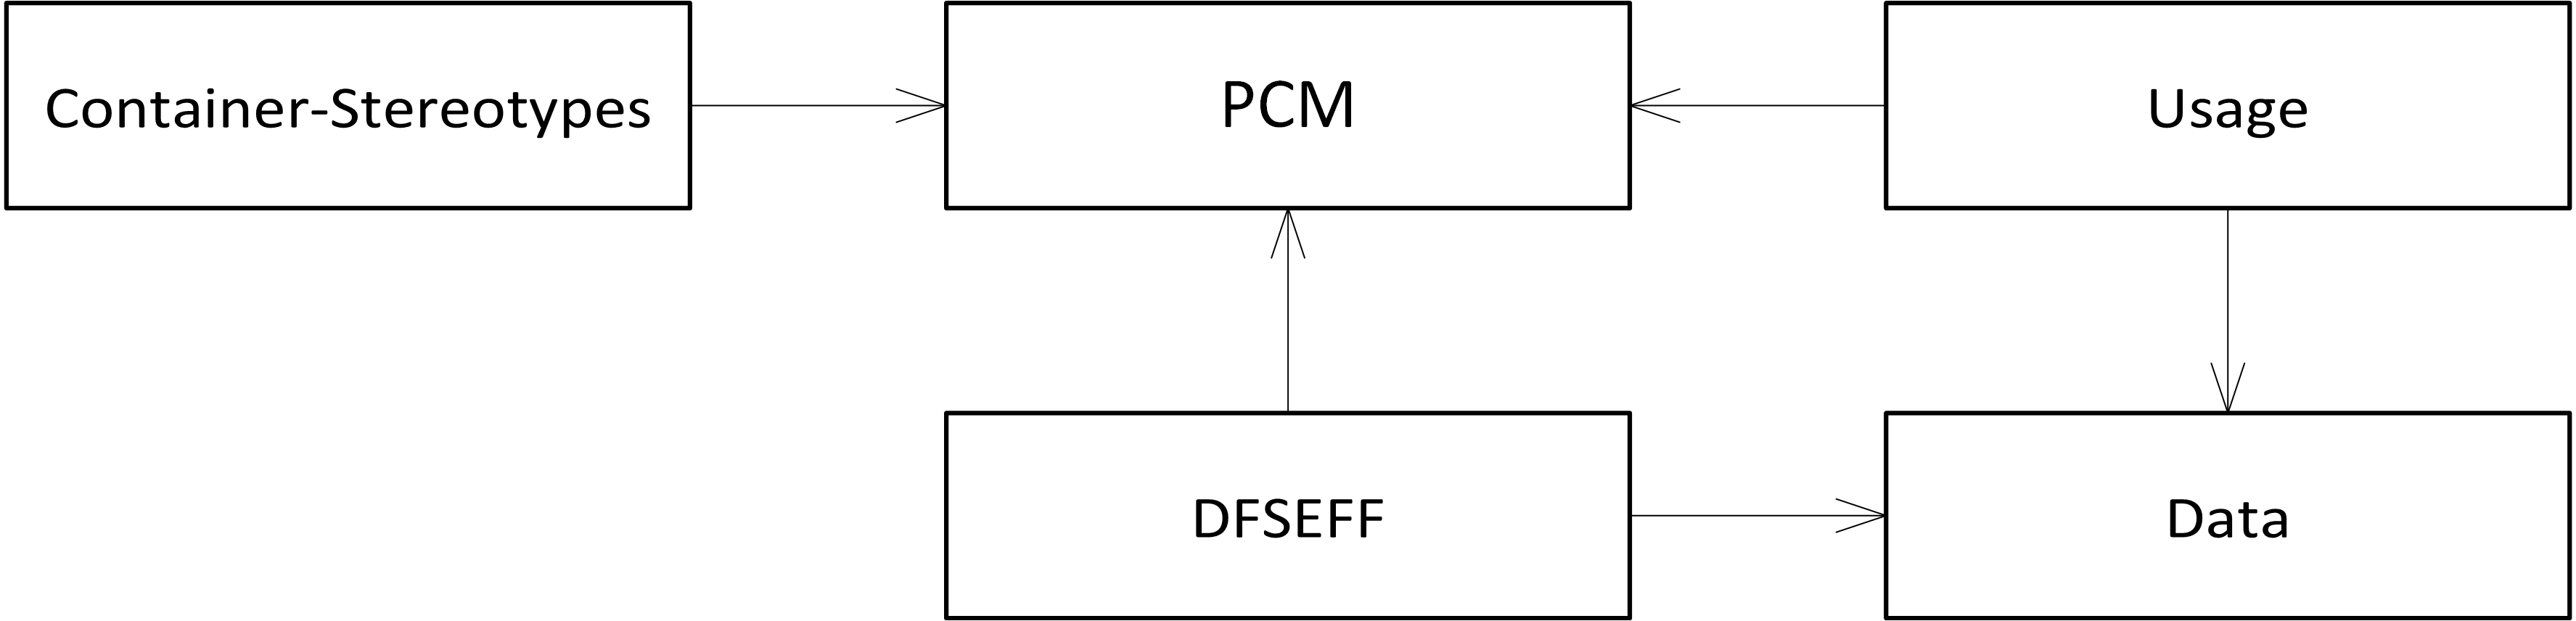
\includegraphics[width=1\textwidth]{images/pakete.png}
	\caption{Übersicht der Pakete der Meta-Modell-Erweiterung}
	\label{img:pakete}
\end{figure}

\section{Beispielszenario}
\label{sec:szenario}
Um die im Folgenden beschriebenen Modellierung besser zu veranschaulichen, soll an dieser Stelle ein Szenario beschrieben werden, in das die einzelnen Pakete und Elemente eingeordnet werden können. In \autoref{img:szenario} ist das Szenario abgebildet. In diesem Szenario gibt es einen Laden, der ein Warenlager hat. In diesem Warenlager befinden sich Produkte. Der Laden besteht nur aus dem Besitzer und nur dieser hat Zugang zu dem Warenlager. Wenn ein Kunde in den Laden kommt richtet er seine Kaufbegehren an den Ladenbesitzer und dieser verkauft ihm je nach Verfügbarkeit das gewünschte Produkt. Für diesen Kaufvorgang benötigt der Ladenbesitzer die Kreditkarte des Kunden. Der Geldbetrag wird mithilfe eines Kreditkartenlesegeräts bei der Bank des Kunden eingefordert. Das Kreditkartenlesegerät ist über das Internet mit der Bank verbunden.

\begin{figure}[h]
	\centering
  	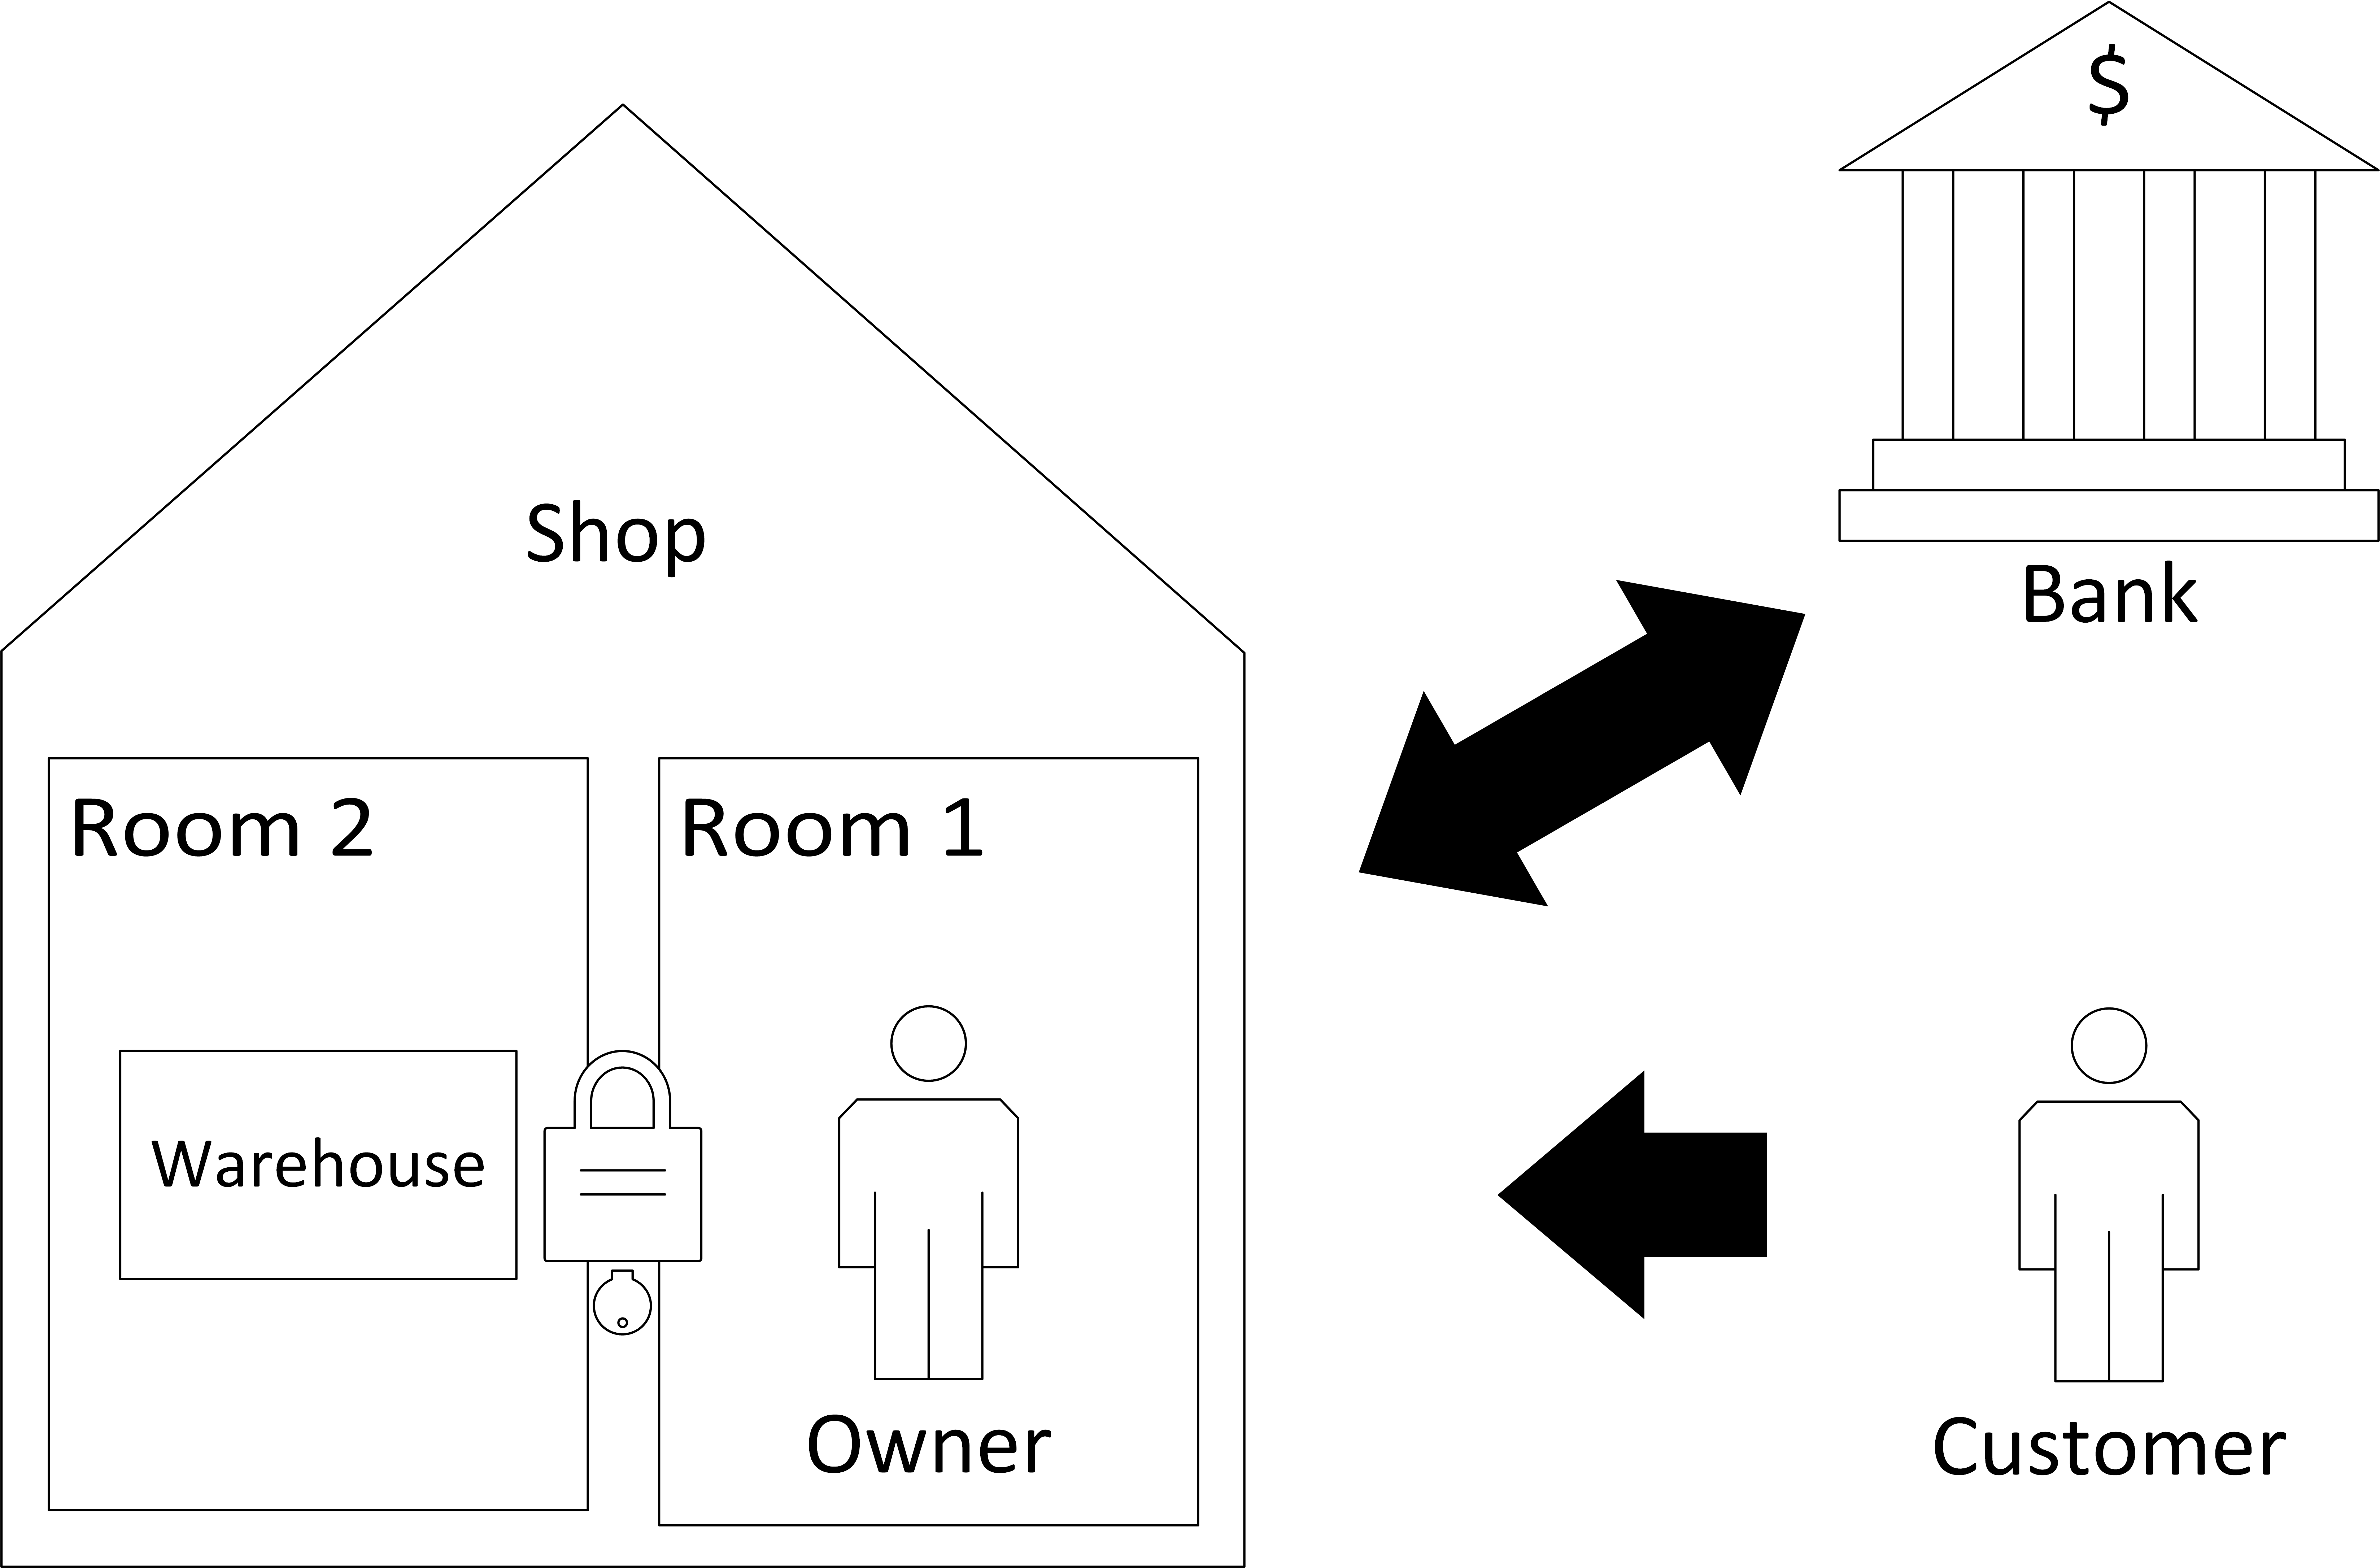
\includegraphics[width=0.6\textwidth]{images/szenario.png}
	\caption{Das Laden-Beispiel-Szenario}
	\label{img:szenario}
\end{figure}

Der Kaufvorgang ist in \autoref{img:szenario:seq} abgebildet. Der Kunde signalisiert dem Besitzer des Ladens, welches Produkt er haben möchte. Der Besitzer prüft nun im Warenlager, ob dieses Produkt vorhanden ist. Ist das der Fall, holt er es heraus und gibt es dem Kunden. Daraufhin bezahlt dieser mit seiner Kreditkarte. Dies ist nur der Basis-Kaufvorgang. Es gibt noch weitere Abläufe, die hier nicht beschrieben werden, wie z.B., wenn das Produkt nicht vorhanden ist.

\begin{figure}[h]
	\centering
  	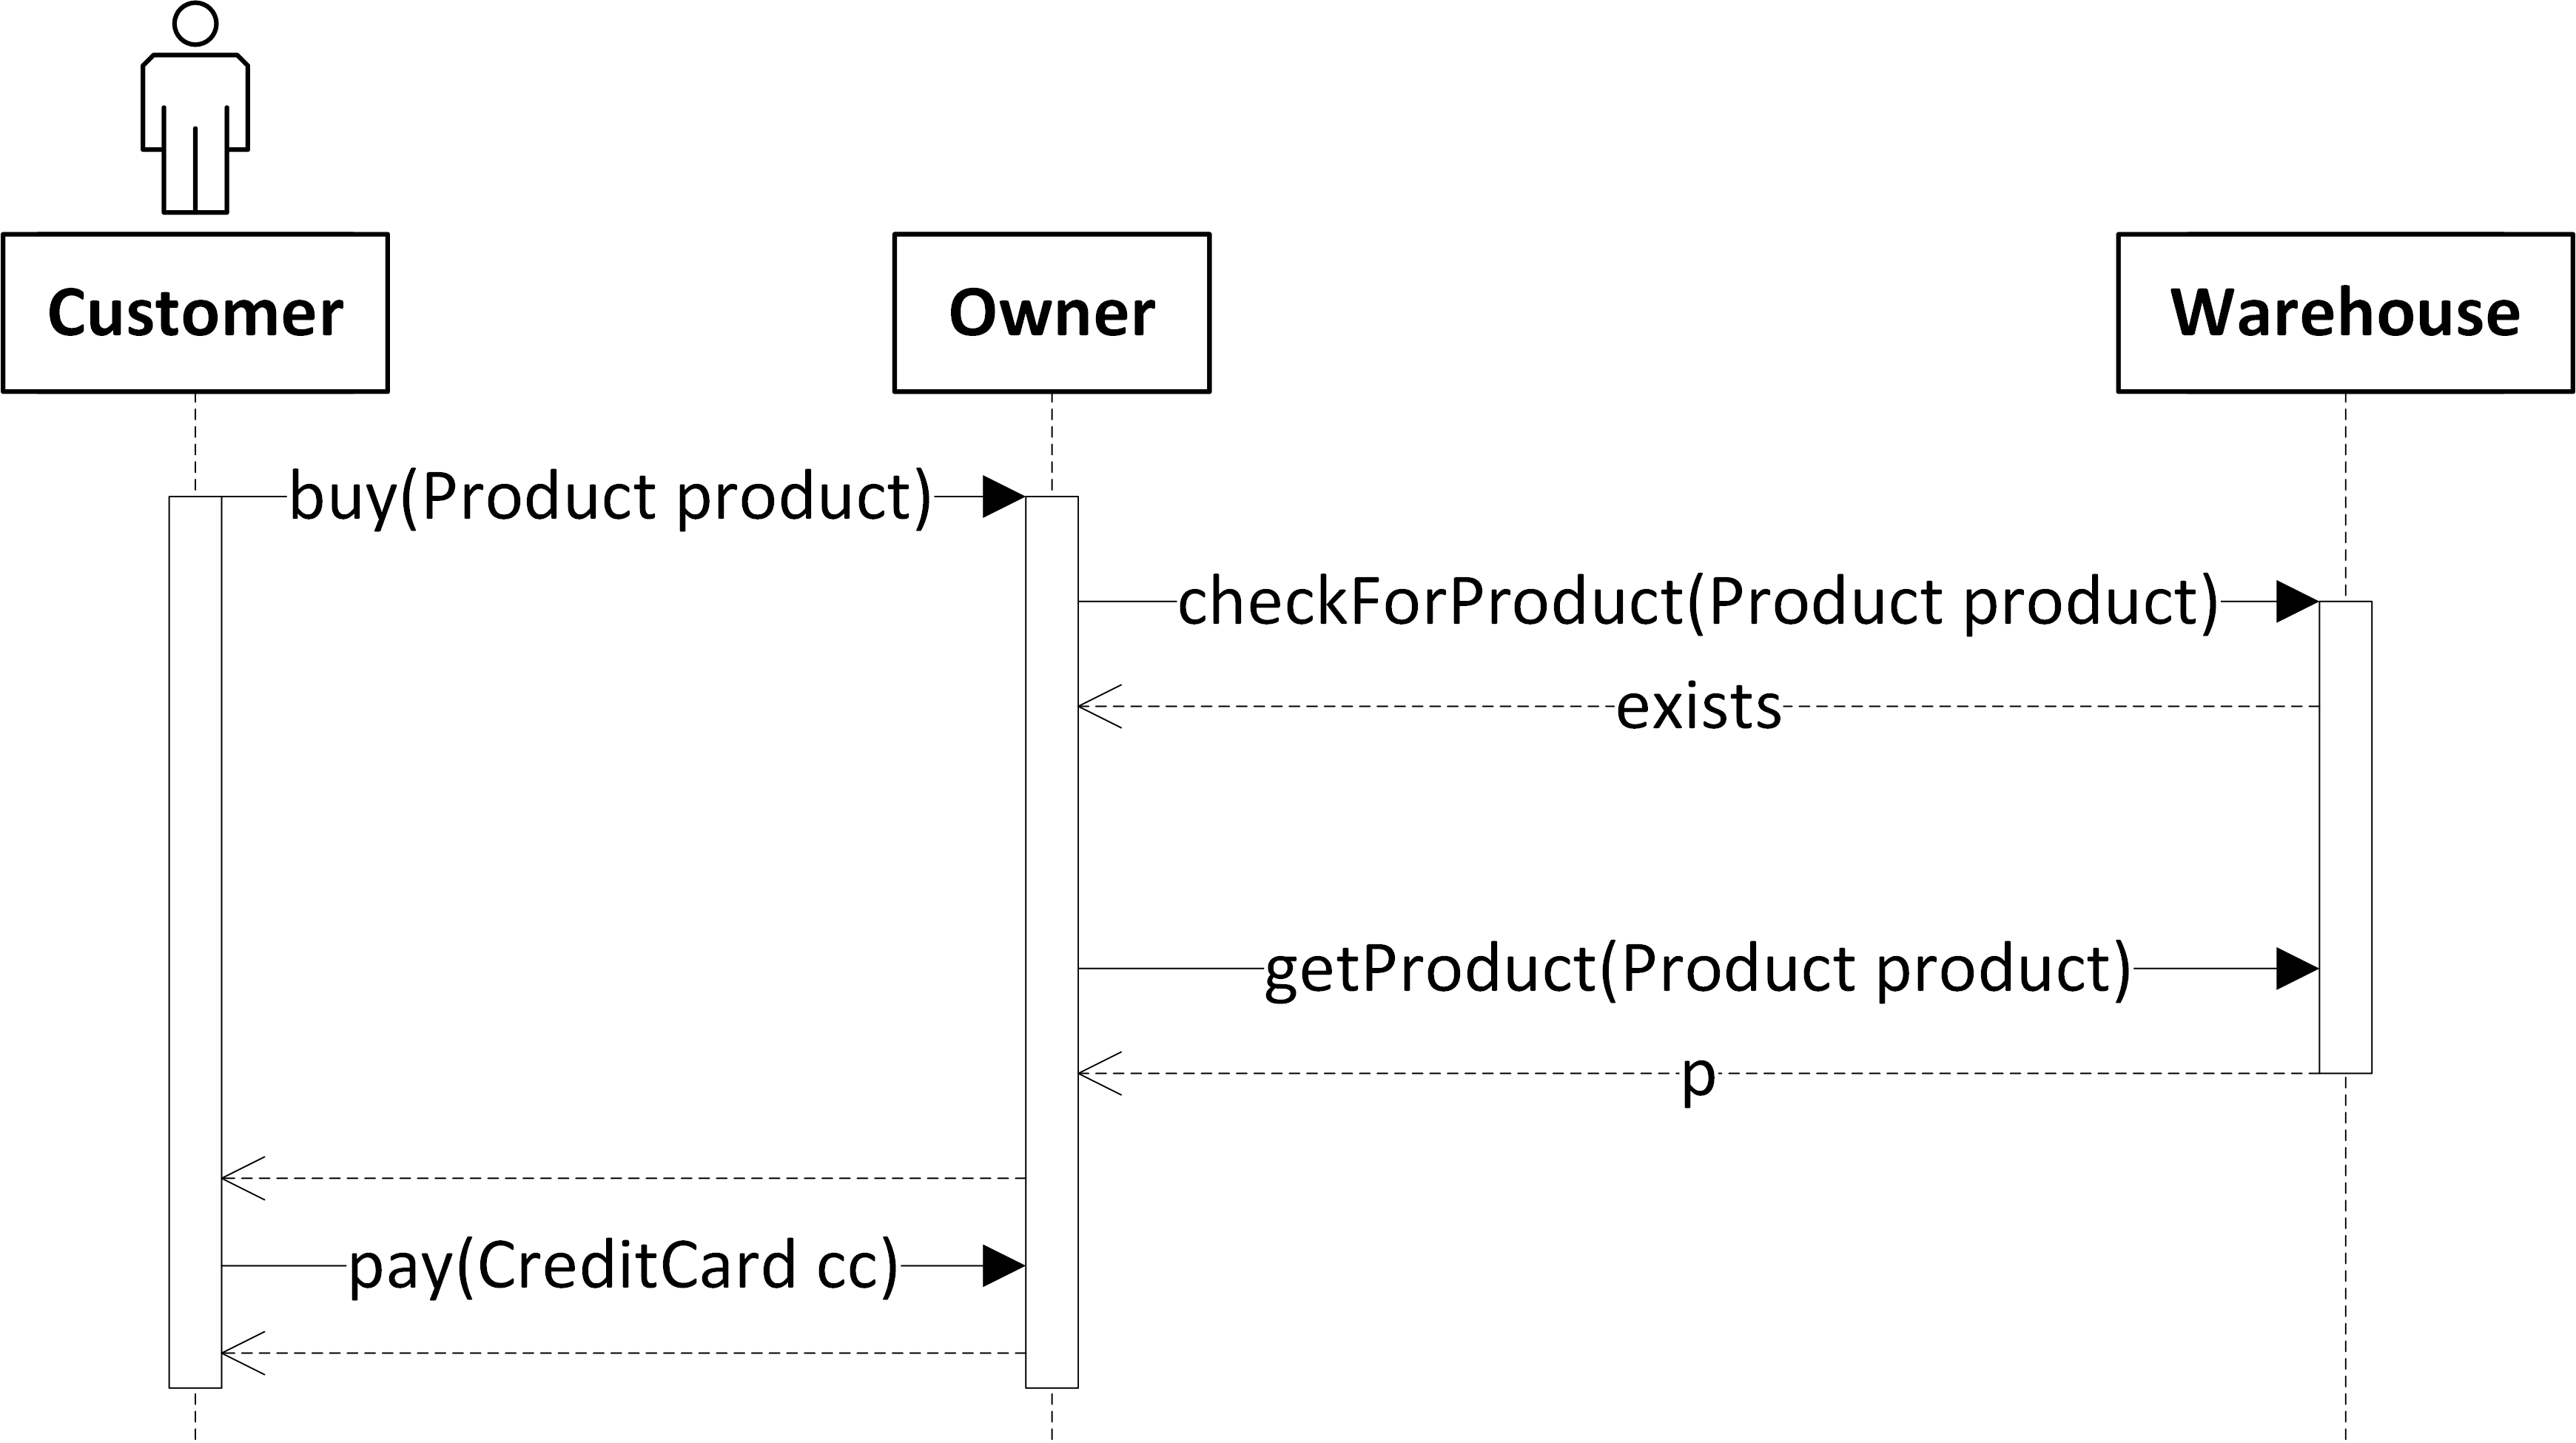
\includegraphics[width=1\textwidth]{images/szenario_seq.png}
	\caption{Der Ablauf eines Basis-Kaufvorgangs im Laden}
	\label{img:szenario:seq}
\end{figure}

\section{Software-Verteilungsexperte}
\label{sec:stereotypes}
Im folgenden wird die Erweiterung des Ressourcen-Umgebungs-Modells vorgestellt. Mithilfe dieser Erweiterung lassen sich die Linking-Resource oder der Resource-Container um verschiedene Eigenschaften erweitern. Die hier beschriebenen Eigenschaften stammen aus \cite{Kramera}, um Vertraulichkeit auf Hardware-Ebene zu unterstützen. Die Eigenschaften werden vom Softwareverteilungsexperten erstellt und referenzieren Resource-Container und Linking-Resources im Execution-Environment-Modell. Eine Darstellung des Modells ist in \autoref{img:modell:stereotypes:übersicht} abgebildet. \par
Damit in Zukunft weitere Eigenschaften hinzugefügt werden können, haben diese eine gemeinsame Oberklasse. Dadurch ist Erweiterbarkeit möglich. Dabei haben die Eigenschaften des Resource-Containers und der Linking-Resources jeweils eine eigene Oberklasse. Außerdem erweitern die Eigenschaften nicht direkt den Resource-Container bzw. die Linking-Resource, sondern werden in einem Container-Element gesammelt und dieser verweist auf den jeweiligen Resource-Container, bzw. die jeweilige Linking-Resource. Dies hat außerdem den Vorteil, dass mehrere Container auf einen Resource-Container oder eine Linking-Resource verweisen können und somit Eigenschaften gruppiert werden können. Nicht benötigte Gruppen können dann bei Bedarf ein- oder ausgeblendet werden. \par
\begin{figure}[h]
	\centering
  	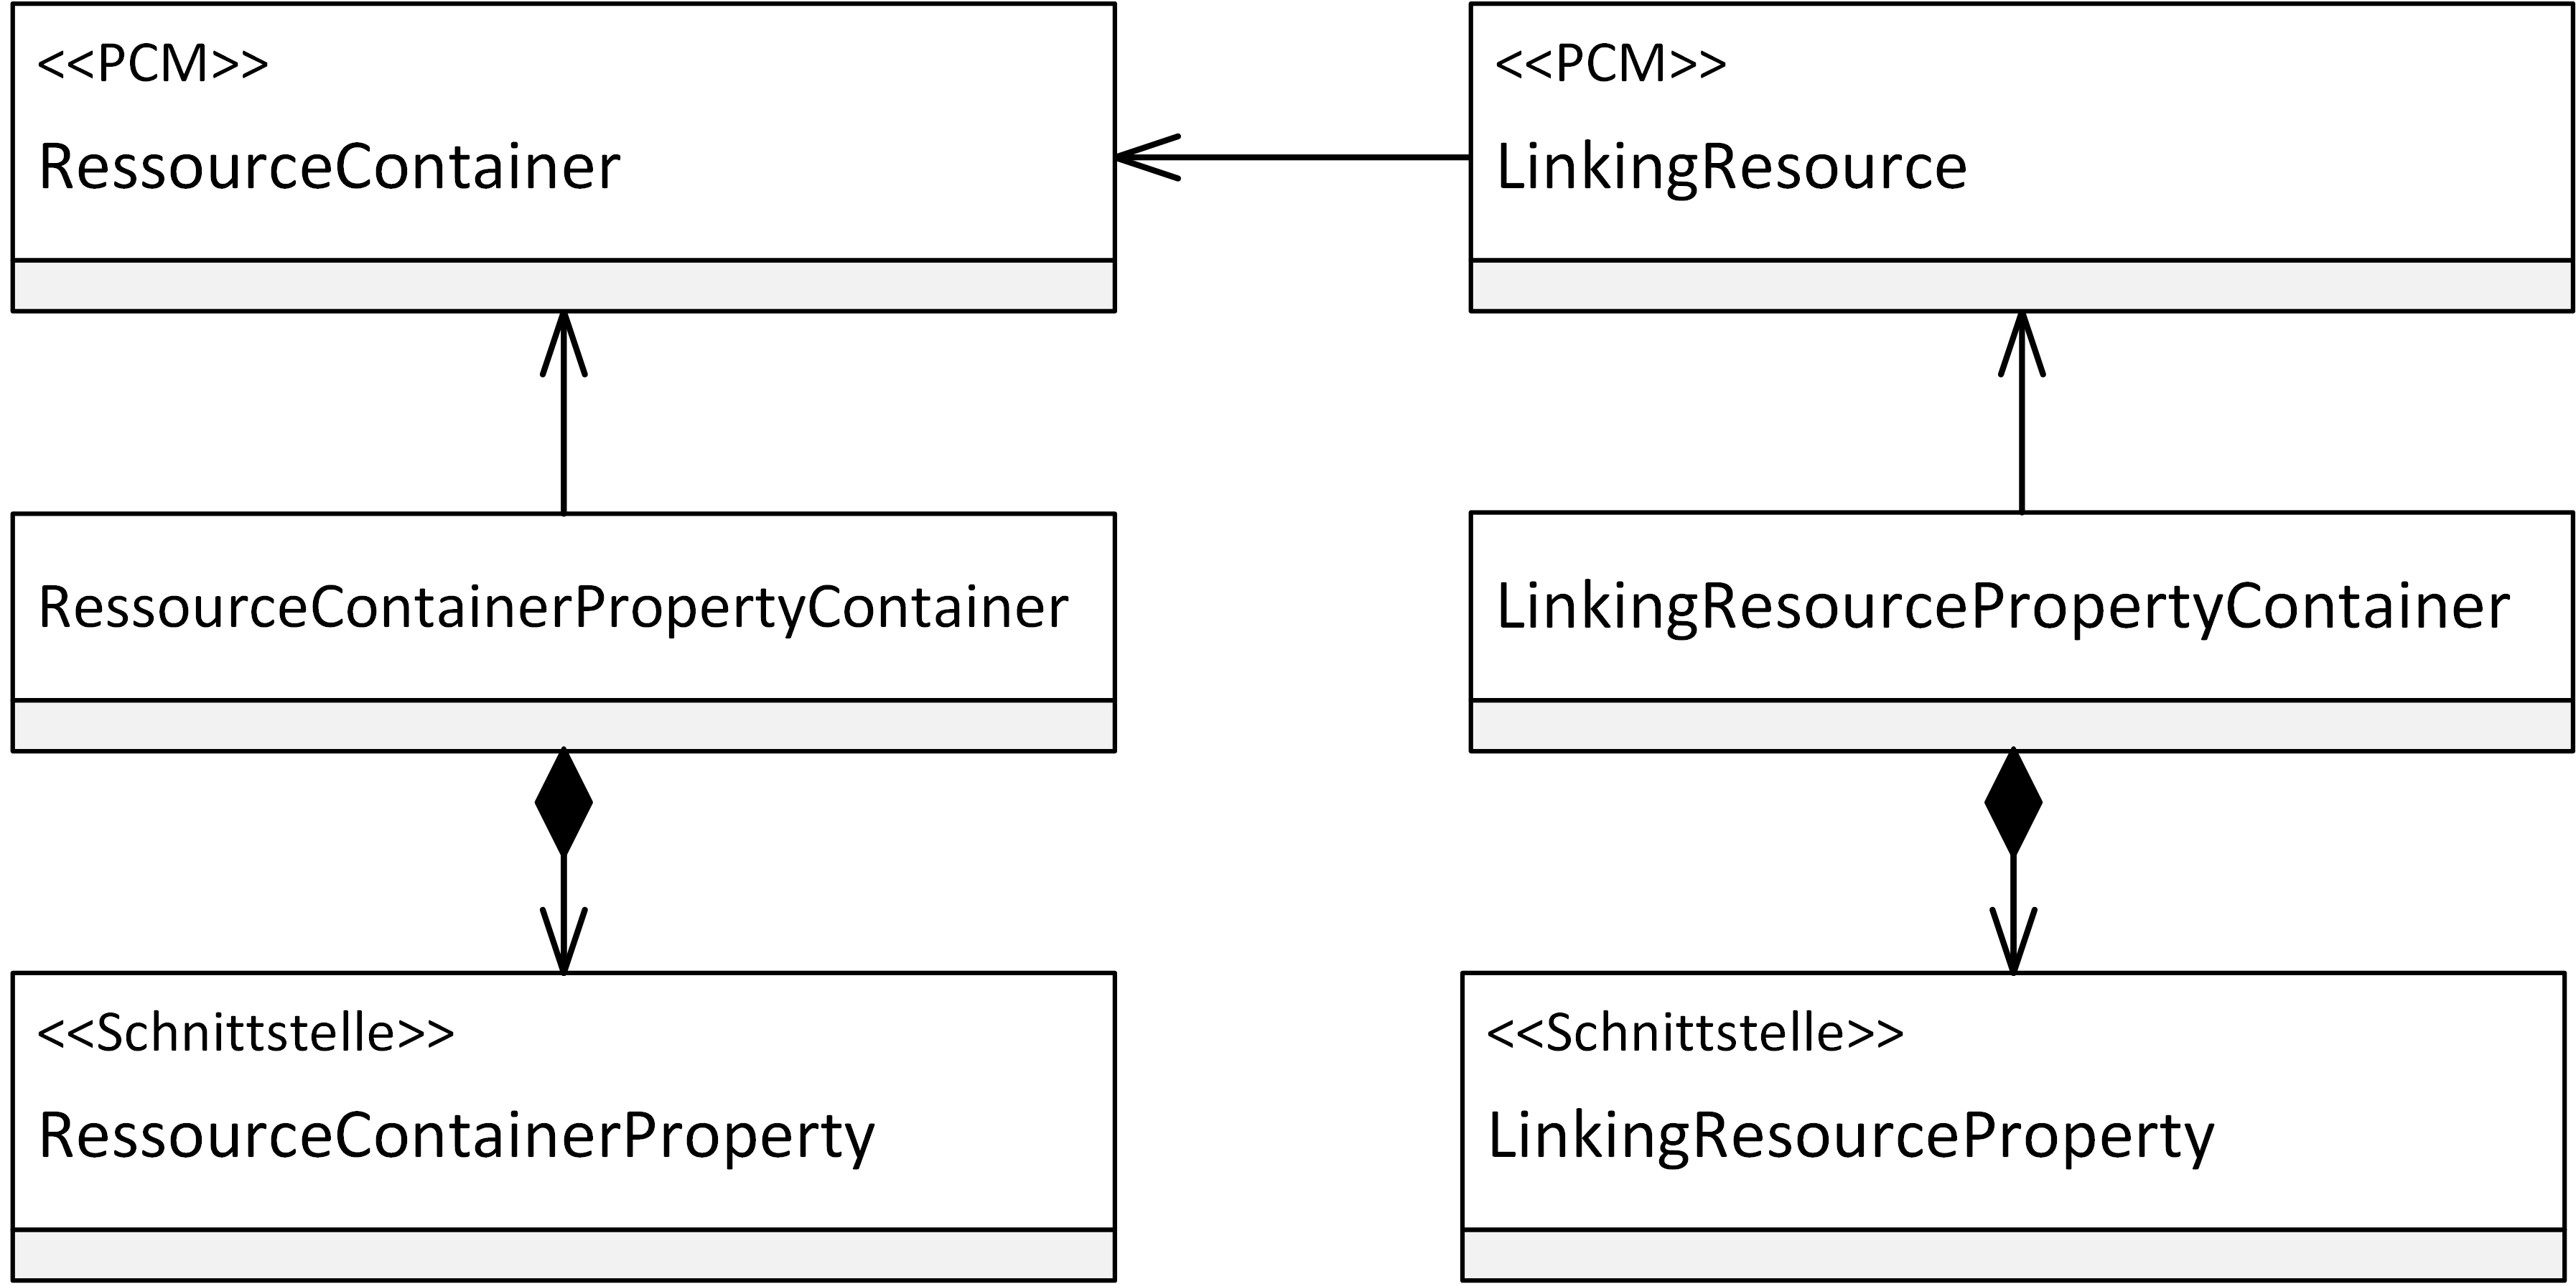
\includegraphics[width=0.75\textwidth]{images/meta_stereotypes_ubersicht.png}
	\caption{Übersicht der Erweiterung für das Ressourcen-Umgebungs-Modell}
	\label{img:modell:stereotypes:übersicht}
\end{figure}
Die Eigenschaften, die einen Resource-Container erweitern können sind in Abbildung \ref{img:modell:stereotypes:properties} abgebildet. Zu diesen Eigenschaften gehört die \texttt{Runtime}-Eigenschaft. Diese Eigenschaft sagt aus, ob auf dem Resource-Container noch weitere Software genutzt wird oder ob alles modelliert wurde. Um das zu spezifizieren, gibt es zwei Optionen. Diese werden in der Aufzählung \texttt{Runtime} modelliert. Wenn weitere Software auf dem Resource-Container genutzt wird, kann das mit \textit{shared} modelliert werden. Wenn aber keine weitere Software auf dem Resource-Container genutzt wird, kann dies mit \textit{exclusive} modelliert werden. Möchte man angeben wo sich ein Resource-Container befindet, erweitert man diesen mit der \texttt{Location}-Eigenschaft. Möchte man den Resource-Container mit einem Sicherheitsmechanismus schützen, erweitert man diesen mit der Eigenschaft \texttt{TamperProtection}. Dadurch lässt sich ein Sicherheitsmechanismus spezifizieren, der den Resource-Container vor Angriffen schützen soll. \par
\begin{figure}[h]
	\centering
  	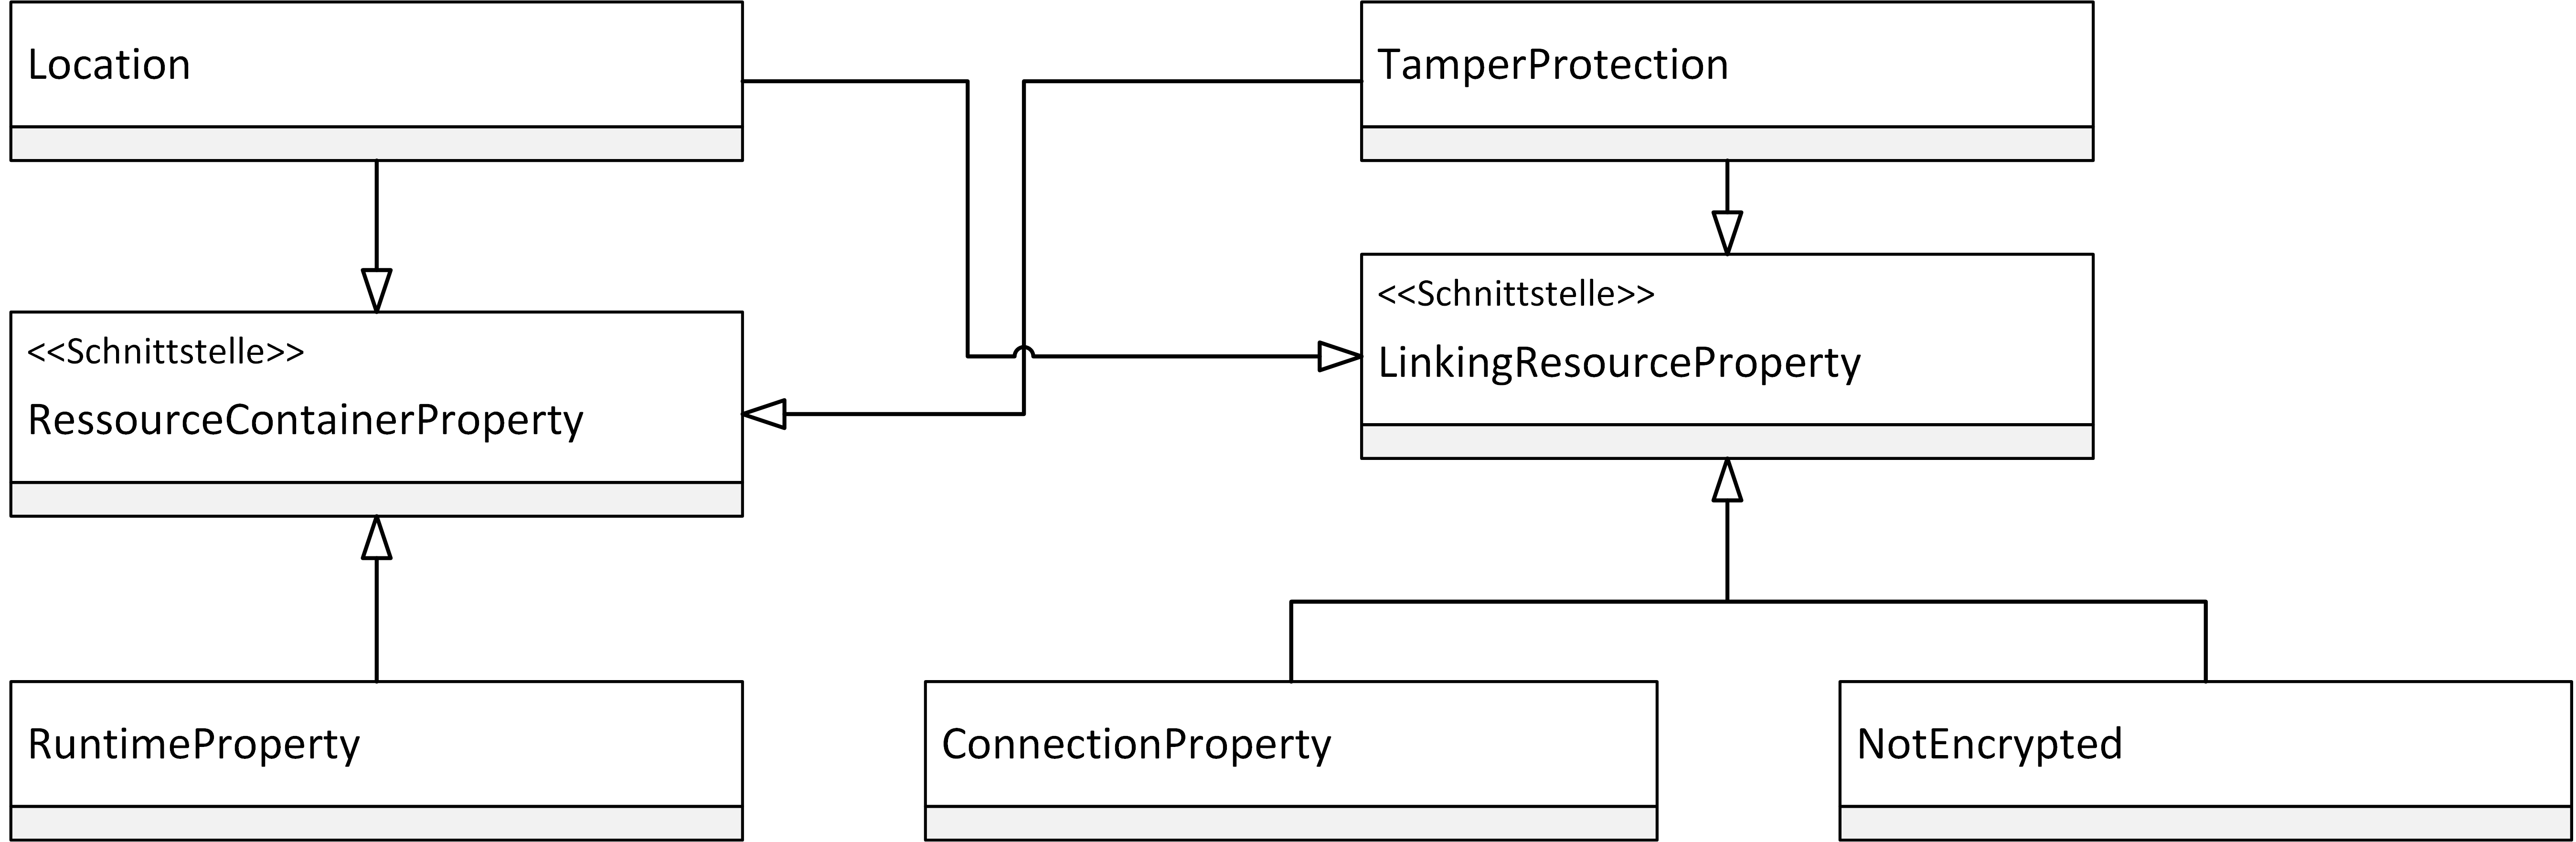
\includegraphics[width=1\textwidth]{images/meta_stereotypes_properties.png}
	\caption{Übersicht der Eigenschaften für Resource"=Container und Linking"=Resource}
	\label{img:modell:stereotypes:properties}
\end{figure}
In \autoref{img:szenario:rc} ist eine mögliche Modellierung eines Resource-Containers des Beispiels aus \autoref{sec:szenario} dargestellt. 
Dabei ist das Kreditkartenlesegerät (\textit{CCReader}) als Resource-Container modelliert. Auf den Resource-Container verweist ein \\\texttt{ResourceContainerPropertyContainer}. Dieser sammelt alle Eigenschaften, die an das Kreditkartenlesegerät angehängt werden sollen. Dazu gehört die \texttt{Runtime}-Eigenschaft. Sie ist hier \textit{exclusive}, da keine weitere Software auf dem Kreditkartenlesegerät genutzt wird. Eine weitere Eigenschaft, die angehängt wird, ist  \texttt{TamperProtection}. Das Kreditkartenlesegerät wird mit einem Passwort vor unbefugten Zugang geschützt. Schließlich wird mit der \texttt{Location}-Eigenschaft festgelegt, dass das Kreditkartenlesegerät sich im zweiten Raum des Ladens befindet. 

\begin{figure}[h]
	\centering
  	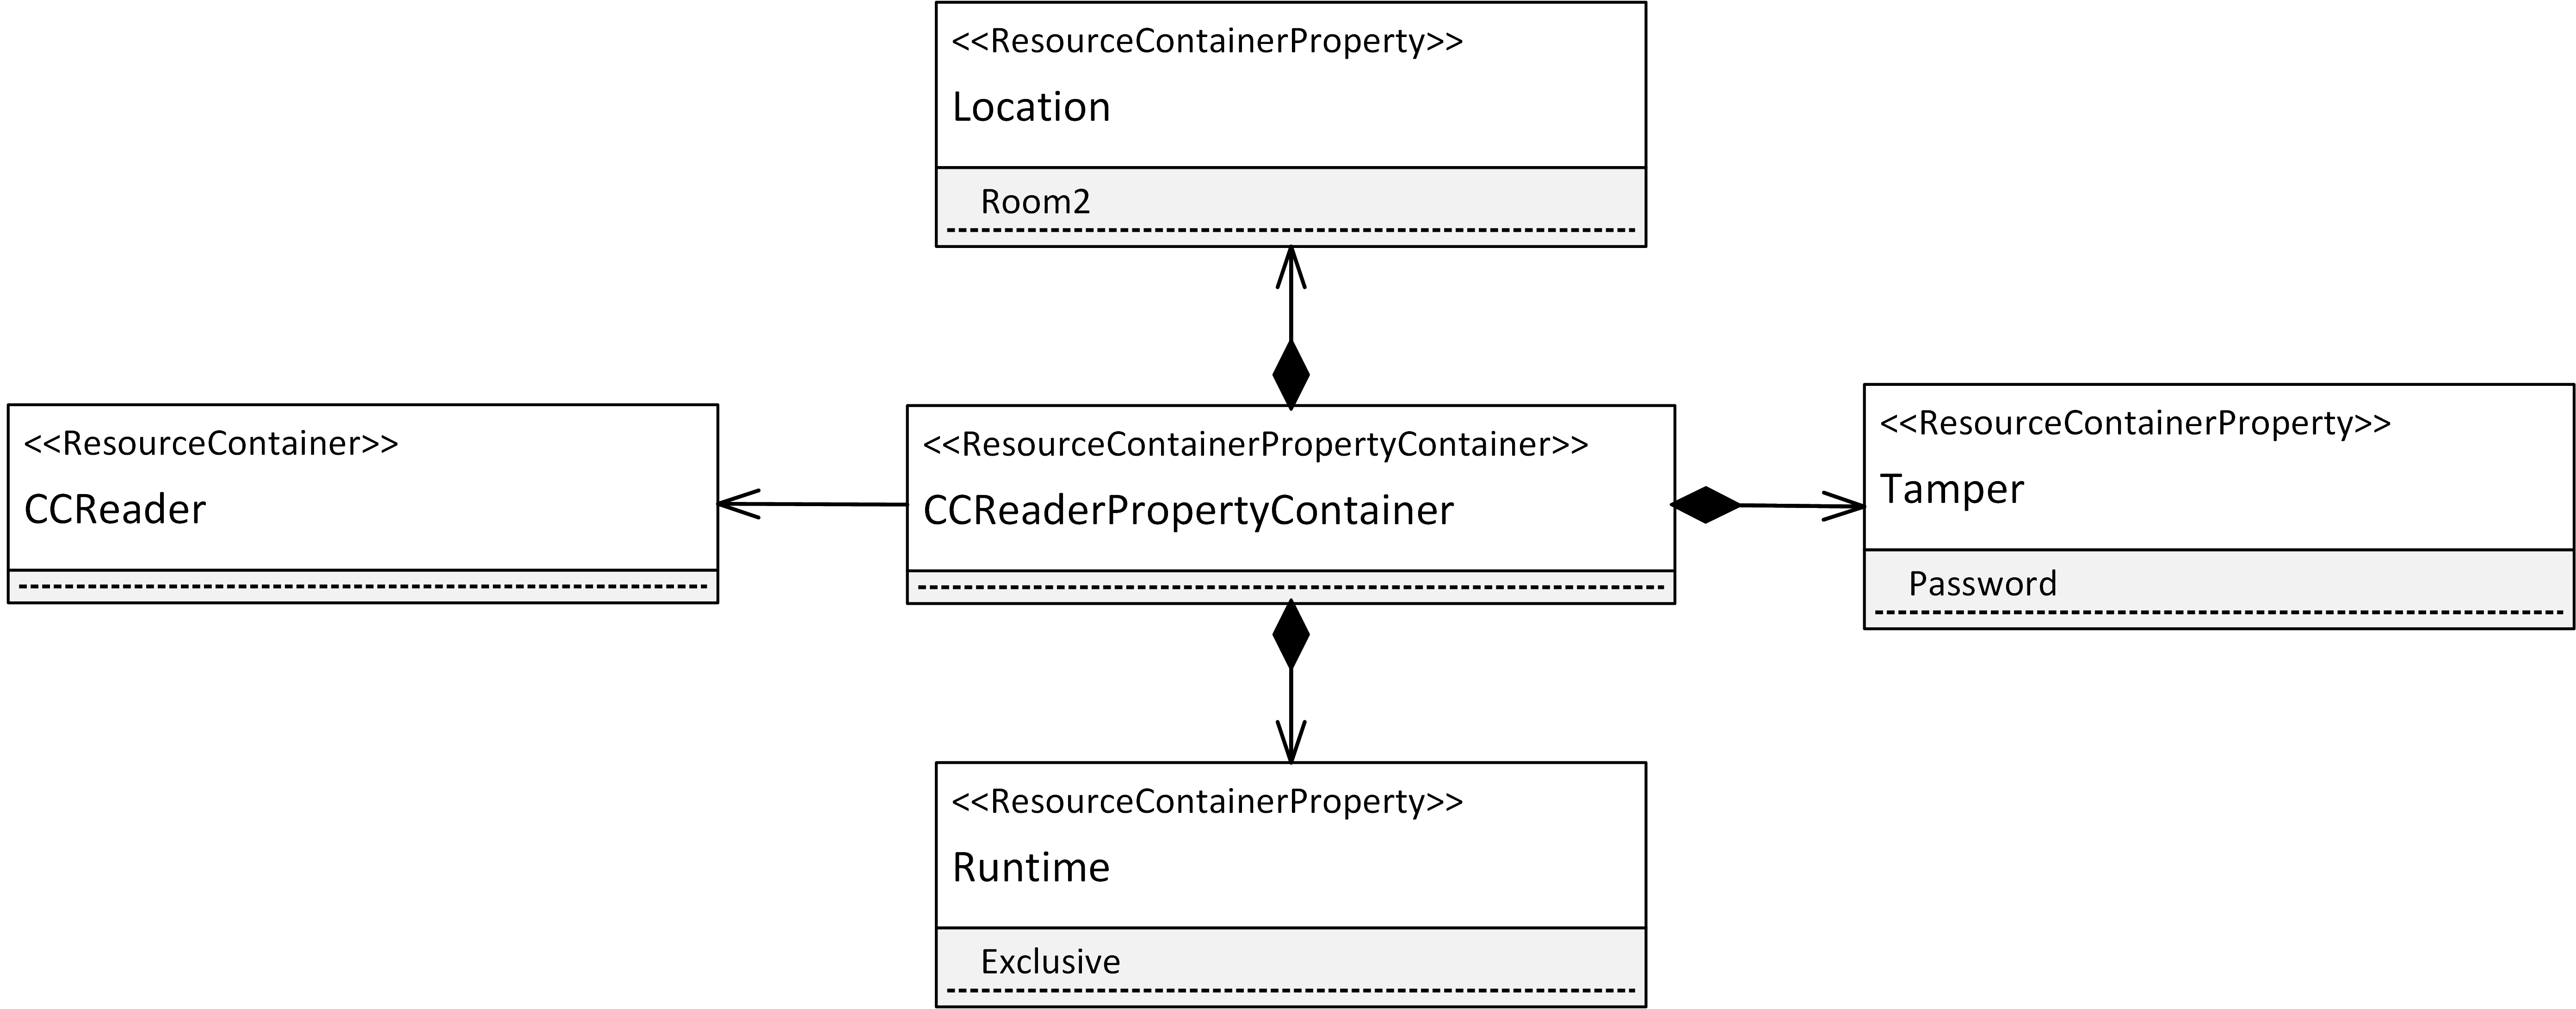
\includegraphics[width=1\textwidth]{images/szenario_rc.png}
	\caption{Resource-Container Beispiel des Laden-Szenarios}
	\label{img:szenario:rc}
\end{figure}

Auch die Linking-Resource kann mit Eigenschaften erweitert werden. Diese sind auch in \autoref{img:modell:stereotypes:properties} abgebildet. Eine Eigenschaft, die Linking-Resource erweitern kann, ist \texttt{Connection}. Diese Eigenschaft gibt an, ob es weitere Verbindungen auf der Linking"=Resource gibt, die aber nicht modelliert wurden. Die Optionen die dabei angegeben werden können sind in der Aufzählung \texttt{Connection} modelliert. Mit \textit{complete} wird signalisiert, dass es keine weiteren Verbindungen gibt. Wenn es weitere Verbindungen gibt, die nicht modelliert wurden, kann dies mit \textit{existing} modelliert werden. Schließlich kann ein Resource-Container Ports enthalten, die nicht verwendet werden, aber eine Verbindung an diesem möglich wäre. Dies kann mit \textit{possible} modelliert werden. Die Eigenschaft \texttt{NotEncrypted} gibt an, ob etwas auf der Linking-Resource nicht verschlüsselt wird, z.B. Protokolle oder Datengröße. Die beiden Eigenschaften \texttt{Location} und \texttt{TamperProtection} sind analog zum Resource-Container. \par
In \autoref{img:szenario:lr} ist eine mögliche Modellierung einer Linking-Resource des Beispiels aus \autoref{sec:szenario} abgebildet. Hier ist die Internetverbindung zwischen dem Kreditkartenlesegerät des Ladens und der Bank des Kundens als Linking-Resource modelliert. Auf die Linking-Resource verweist ein \texttt{LinkingResourcePropertyContainer}. Dieser sammelt alle Eigenschaften, die an die Linking-Resource angehängt werden sollen. Dazu gehört die \texttt{Location}-Eigenschaft. Sie spezifiziert als Ort, für die Linking-Resource, das Internet. Geschützt ist die Linking-Resource mit einem Passwort. Dies ist in der Eigenschaft \texttt{TamperProtection} spezifiziert. Außerdem wird spezifiziert, dass das Protokoll, über das kommuniziert wird, nicht verschlüsselt wird. Mithilfe der Eigenschaft \texttt{NotEncrypted} wird dies modelliert. Schließlich wird mit der \texttt{Connection}-Eigenschaft angegeben, dass es keine weiteren Verbindungen, außer den modellierten gibt (\textit{complete}). 

\begin{figure}[h]
	\centering
  	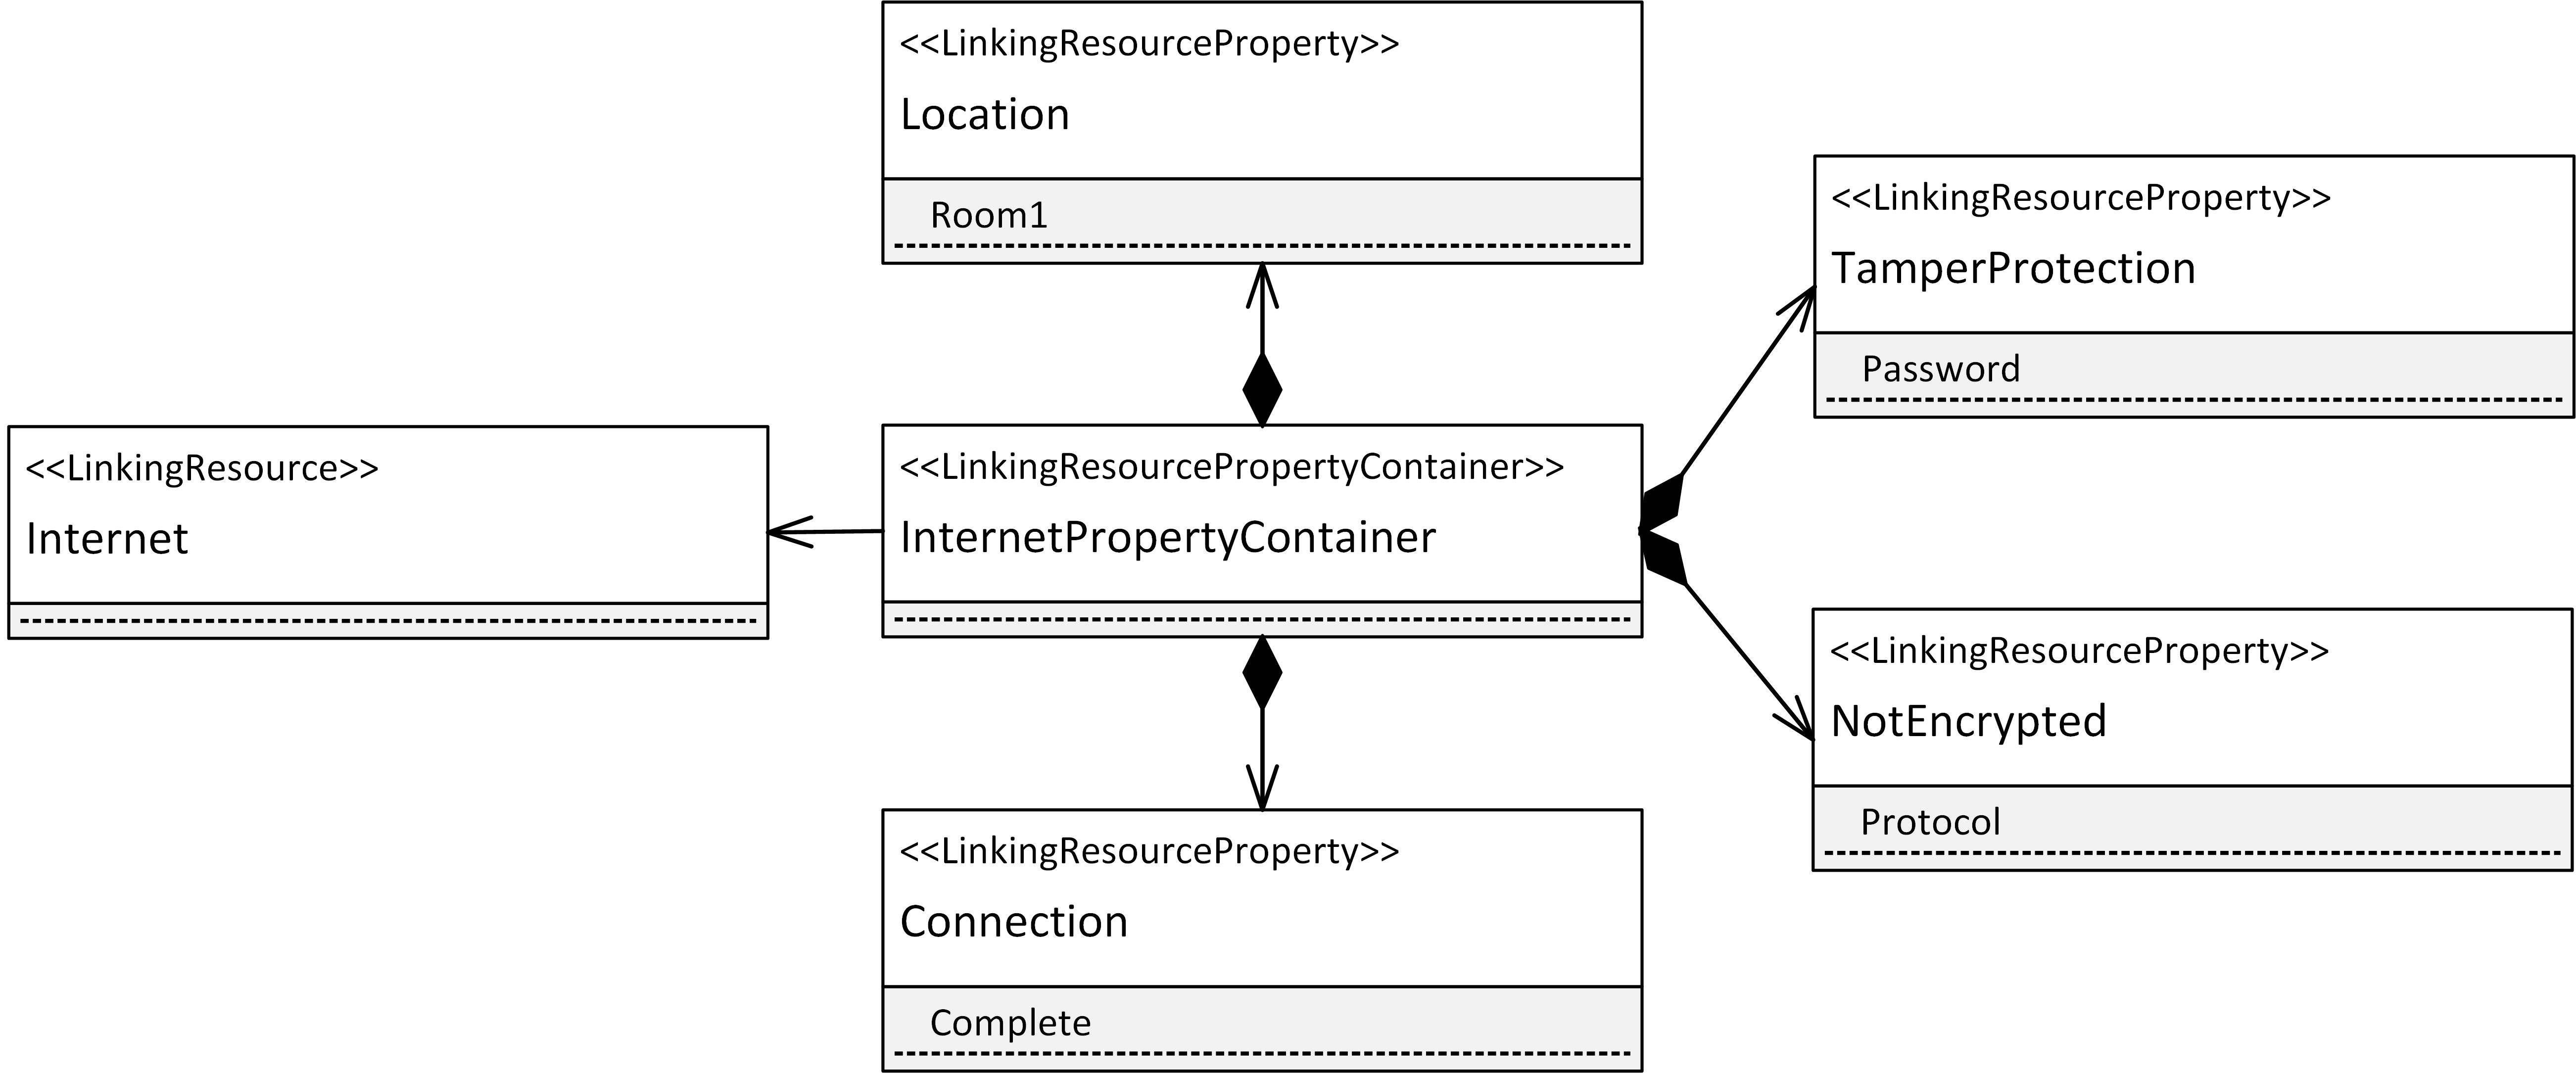
\includegraphics[width=1\textwidth]{images/szenario_lr.png}
	\caption{Linking-Resource Beispiel des Laden-Szenarios}
	\label{img:szenario:lr}
\end{figure}

\section{Datenmodellierer}
\label{sec:data}
In diesem Abschnitt, wird die Modellierung von Daten beschrieben, die in einem System verarbeitet werden. Dabei handelt es sich nicht um individuelle Daten, sondern um Datenklassen. Das können z.B. Daten sein, die für einen Kauf benötigt werden, wie Name oder Adresse. Das bedeutet, dass der Benutzer die Datenklasse \texttt{Namen} in den Dienst eingibt und nicht einen speziellen Namen. Die Daten werden vom Komponentenentwickler sowie dem Domänenexperten im Ressourcen-Umgebungs-Modell und Nutzungsmodel eingesetzt. In \autoref{img:modell:data} ist diese Modellierung abgebildet. \par
Die Klasse \texttt{Data} repräsentiert dabei eine Datenklasse. An \texttt{Data} können Eigenschaften (\texttt{DataProperty}) angehängt werden. Mithilfe eines \texttt{DataPropertyContainers} werden die Eigenschaften gesammelt und an eine Datenklasse gehängt. Die Eigenschaften können je nach untersuchtem Qualitätsattribut unterschiedlich sein. Sie können daher variabel gewählt werden. Für Datenflussanalysen können so Sicherheitseigenschaften spezifiziert werden. Darauf aufbauend ist eine Überprüfung der Einhaltung dieser Eigenschaften möglich. Außerdem befindet sich in dem Paket das Element \texttt{DataSet}. Ein \texttt{DataSet} ist eine Gruppierungen von Datenklassen. Daten können so verschiedene Gruppierungen zugeordnet werden. Im Anschluss kann, in Hinblick auf eine Datenflussanalyse, festgelegt werden, welche Person Zugriff auf welche \texttt{DataSet}s haben soll. Während der Datenflussanalyse kann schließlich geprüft werden, ob jeder nur Zugriff auf die \texttt{DataSet}s hat, auf die er zugreifen darf. \par
\begin{figure}[h]
	\centering
  	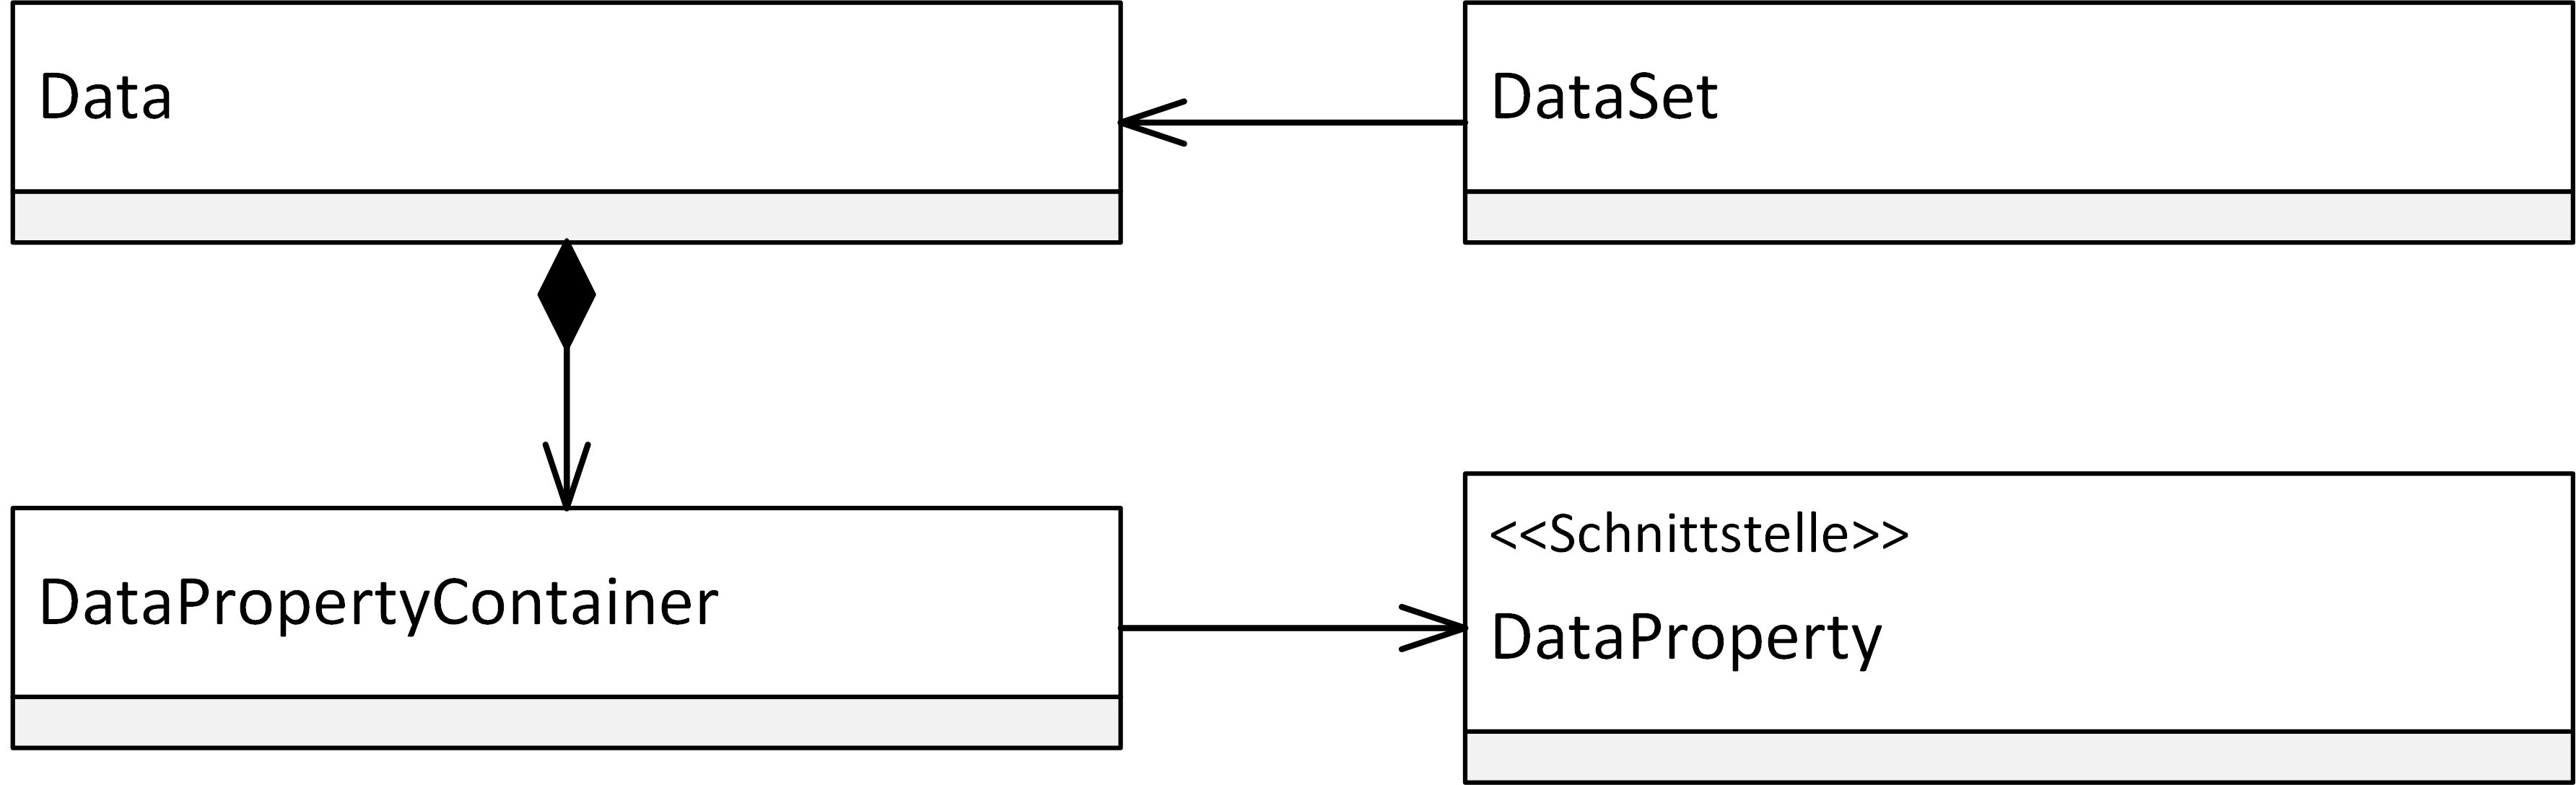
\includegraphics[width=0.8\textwidth]{images/meta_data.png}
	\caption{Übersicht der Datenmodellierung}
	\label{img:modell:data}
\end{figure}
In dem Beispielszenario aus \autoref{sec:szenario} wären \textit{Kreditkartendaten}  eine Datenklasse und \textit{Kunde}, \textit{Besitzer} und \textit{Warenlager} als \texttt{DataSet} modelliert. Dabei sind die \textit{Kreditkartendaten} nur im \texttt{DataSet} \textit{Kunde}. Das heißt, dass nur Personen, die dem \texttt{DataSet} \textit{Kunde} zugewiesen sind, Zugriff auf die Daten haben. Bei einer Datenflussanalyse kann nun geprüft werden, ob die \textit{Kreditkartendaten} bei einer Person oder einem System ankommen, die eigentlich keinen Zugriff auf diese haben sollte. 

\section{Komponentenentwickler}
\label{sec:paket:dfseff}
In diesem Abschnitt wird die Modellierung für einen \gls{dfseff} beschrieben. Mit diesem \gls{dfseff} kann der Komponentenentwickler einen Datenfluss innerhalb einer Komponente, in Form eines \gls{seff}, modellieren. Dabei soll es möglich sein Daten zu verfeinern, indem man diese mit Parametern verknüpft. Außerdem soll der Datenfluss über mehrere Datenverarbeitungsschritte modelliert werden können und schließlich ein globaler Datenfluss aus dem Nutzungs-, Komponenten-Repository-, Ressourcen-Umgebungs-, Komponenten-Allokations- und System-Modell abgeleitet werden. Vor der Meta-Modell-Bildung muss überlegt werden, ob Elemente aus dem \gls{pcm} wiederverwendet werden können. Das war in den Abschnitten davor nicht nötig, da es nichts Vergleichbares in Palladio gab. In Palladio existiert aber bereits ein \gls{seff}. Der \gls{rdseff}, der eine \gls{seff}-Spezialisierung für Performanzvorhersagen darstellt. \par 
Als ein Elemente, das wiederverwendet werden kann, wurde die \texttt{Signatur} identifiziert. Eine \texttt{Signatur} modelliert die Signatur einer Methode. Dazu zählen Parameter, der Rückgabetyp und Fehlerspezifikationen. Der Vorteil dieser Wiederverwendung ist, dass der Komponentenentwickler seine bereits modellierten Signaturen wiederverwenden kann. Außerdem geht der Zusammenhang zwischen Kontroll- und Datenfluss nicht verloren. Ein weiteres Element, das wiederverwendet werden kann, ist \texttt{Parameter}. \texttt{Parameter} modelliert einen Parameter einer \texttt{Signatur}. \texttt{Parameter} besteht aus einem Namen und einem Datentyp.  
Die Vorteile sind ähnlich zu denen der \texttt{Signatur}. \texttt{Parameter} ist nicht vom \gls{rdseff} abhängig. Außerdem geht der Zusammenhang zwischen Kontroll- und Datenfluss nicht verloren. Alternativ wäre hier ein neues Parameter Element möglich, dass direkt Daten und Parameter verknüpft. Jedoch hat bei dieser Modellierung der Benutzer wenig Mehrwert und muss stattdessen evtl. bereits modellierte Parameter neu modellieren. \par
Elemente, die hingegen nicht wiederverwendet werden können, sind \texttt{AbstractAction}, ihre Unterklassen und \texttt{ResourceDemandingBehaviour}. \texttt{AbstractAction} modelliert dabei einen Aufruf zu einem internen oder externen Dienst. Außerdem hat \texttt{AbstractAction} eine Referenz zu \texttt{ResourceDemandingBehaviour}. Dieses Element modelliert das Verhalten einer Komponente als Sequenz von \texttt{AbstractAction}s. Durch die Wiederverwendung der Elemente würden auch eine Vielzahl anderer Elemente im \gls{dfseff} verwendbar werden, die aber an dieser Stelle keinen Sinn machen. Ein Beispiel wäre hier die \texttt{ReleaseAction}, die eine Unterklasse von \texttt{AbstractAction} ist. Die \texttt{ReleaseAction} gibt Ressourcen im \gls{rdseff} wieder frei. Da Ressourcen für die untersuchte Analyse nicht benötigt werden, ist eine Wiederverwendung an dieser Stelle nicht sinnvoll. \par
Eine Übersicht des Meta-Modells ist in \autoref{img:modell:dfseff:übersicht} abgebildet. Das Root-Element, dieser Erweiterung, ist das Element \texttt{DataFlowSEFF}. Aufgrund einer Containment"=Beziehung zwischen den Elementen \texttt{BasicComponent} und \texttt{ServiceEffectSpecification} kann das Element \texttt{ServiceEffectSpecification} nicht wiederverwendet werden. \\\texttt{ServiceEffectSpecification} ist eine abstrakte Klasse und modelliert dabei einen \gls{seff}. Spezielle \gls{seff}s sollten von dieser Klasse erben. Stattdessen referenziert das Element \\\texttt{DataFlowSEFF} die Elemente \texttt{BasicComp-\\onent} und \texttt{Signature}. Eine \texttt{BasicComponent} modelliert in \gls{pcm} eine Komponente. Komponenten können dabei abstrakt oder konkret sein. Abstrakte Komponenten spezifizieren nur ihre Schnittstellen und werden vom Software-Architekten als Platzhalter verwendet. Sie werden im weiteren Verlauf der Bachelorarbeit nicht näher betrachtet. Konkrete Komponenten sind entweder Basis Komponenten (\texttt{BasicComponent}) oder setzen sich aus mehreren zusammen. Eine \texttt{BasicComponent} spezifiziert dabei, für jede Operation die sie bereitstellt, ein Verhalten. Die zusammengesetzten Komponenten werden im Weiteren nicht näher betrachtet. \par 
Außerdem enthält \texttt{DataFlowSEFF} das Element \texttt{DataFlowBehavior}. \texttt{DataFlowBehavior} modelliert das Verhalten einer Komponente als Sequenz, die aus mehreren \texttt{DataFlow-\\AbstractActions} besteht.
\begin{figure}[h]
	\centering
  	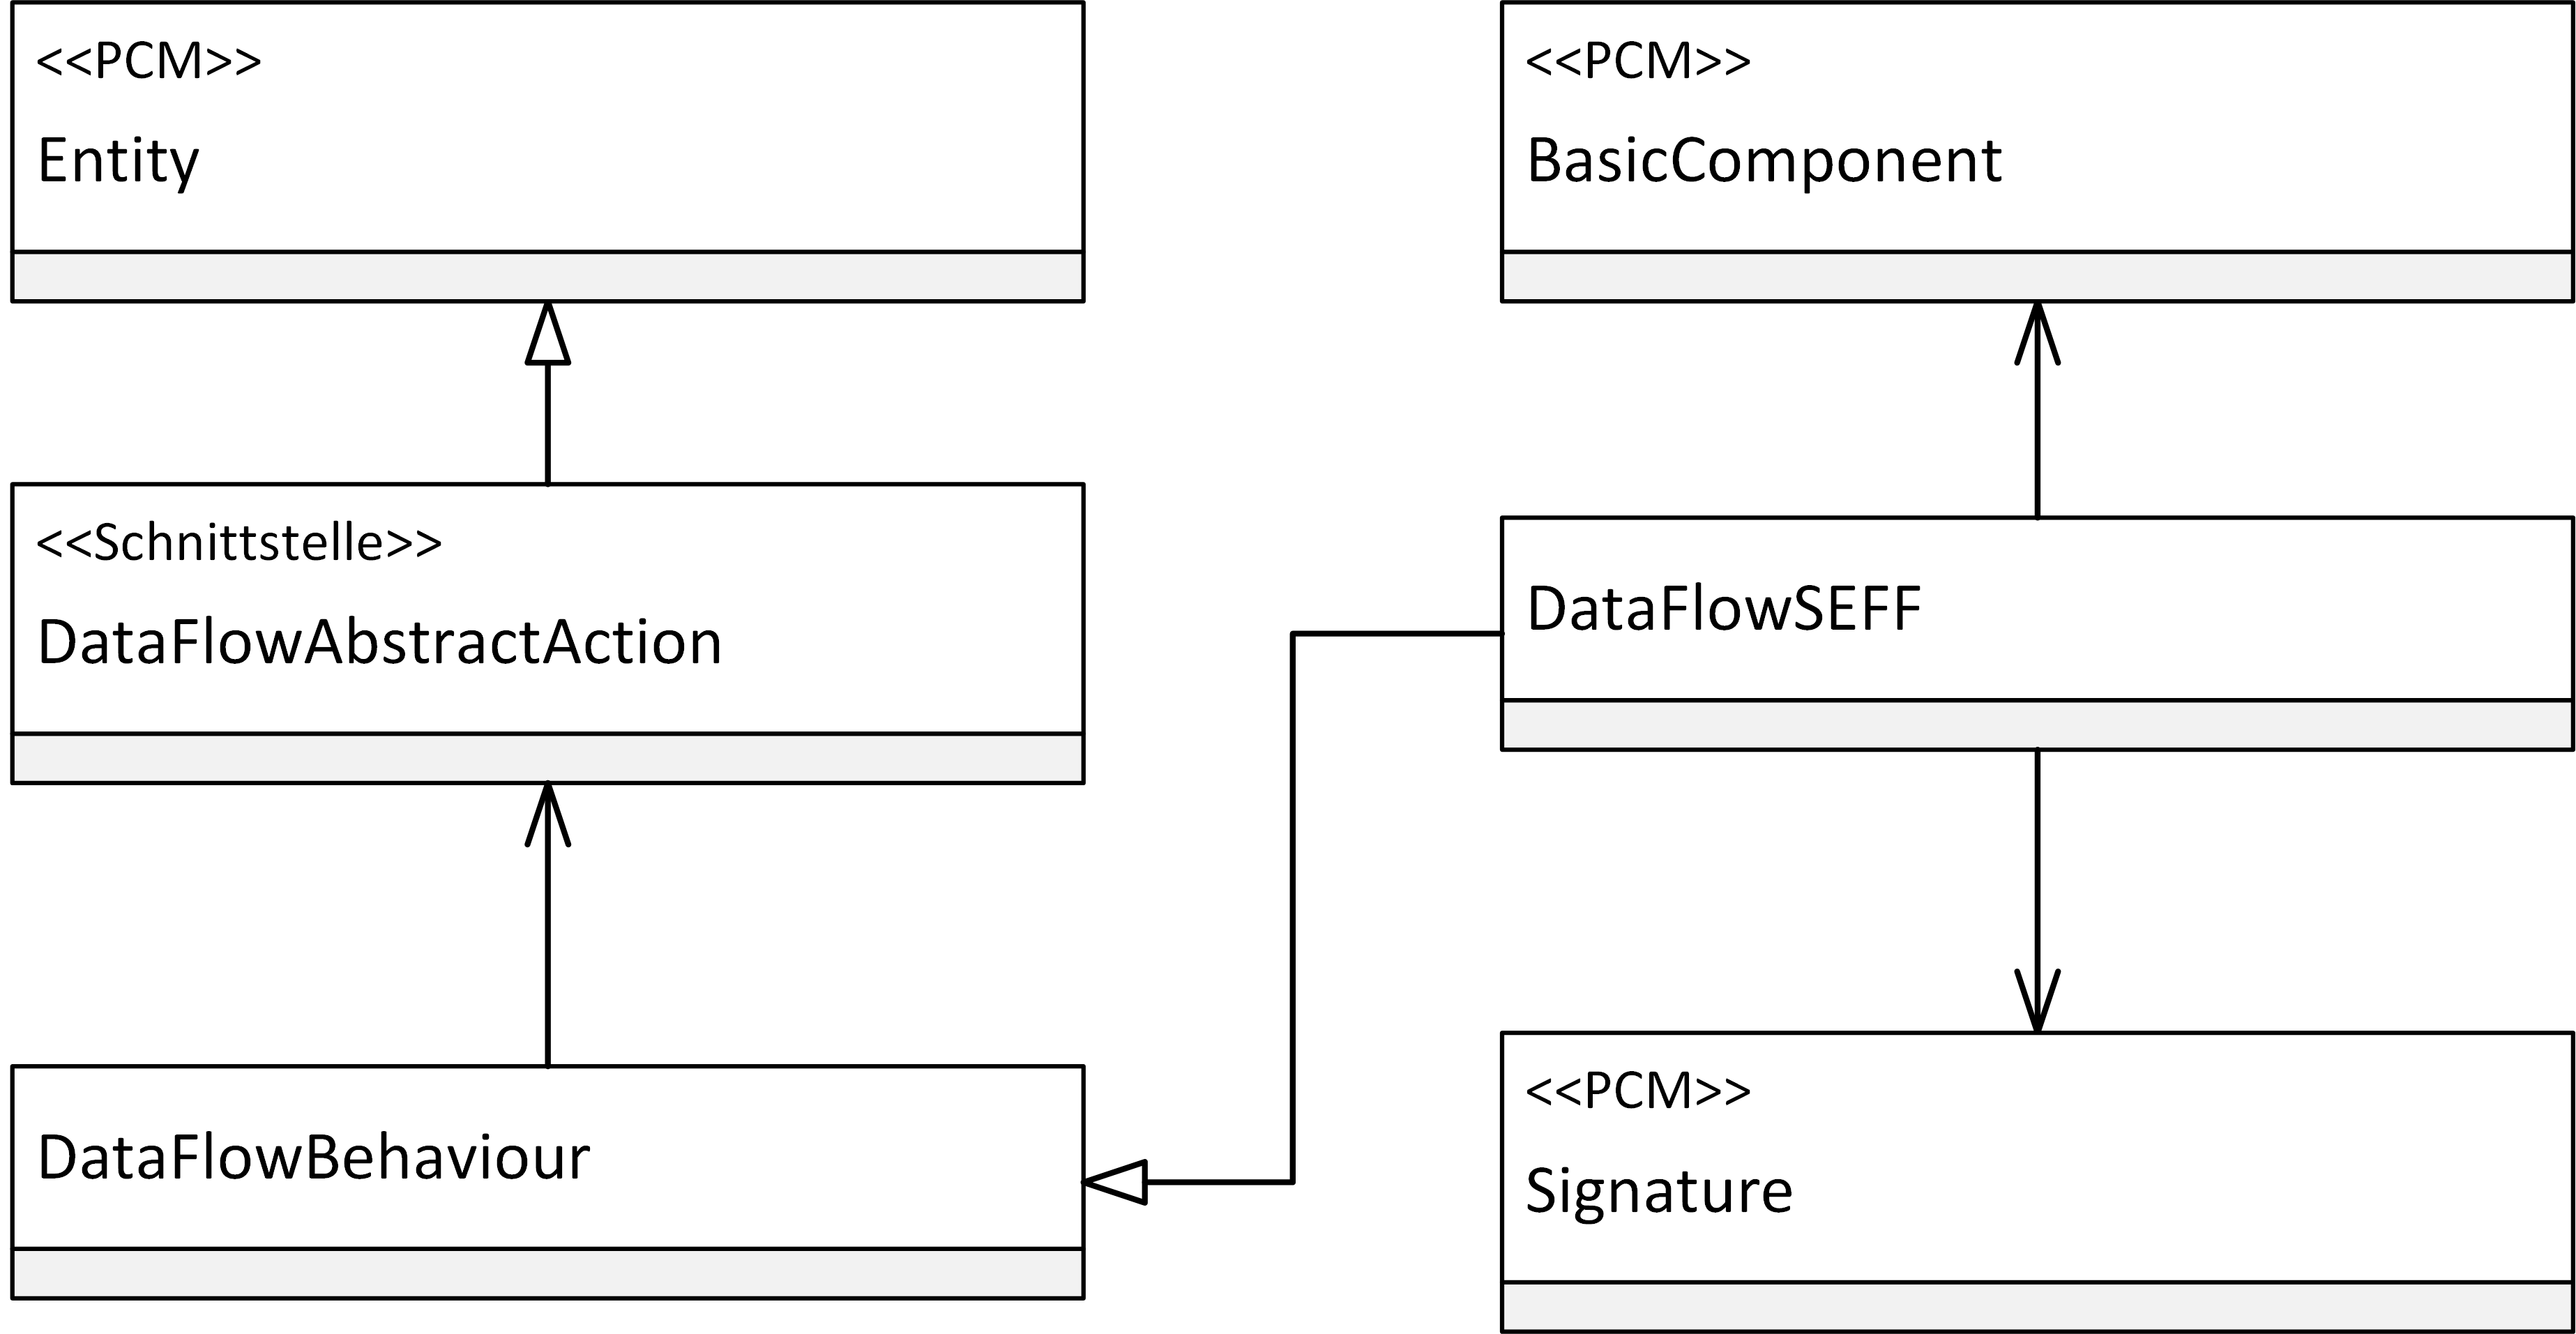
\includegraphics[width=0.8\textwidth]{images/meta_dfseff_ubersicht.png}
	\caption{Übersicht der DFSEFF Erweiterung}
	\label{img:modell:dfseff:übersicht}
\end{figure}
Der Ablauf eines \gls{dfseff} ist ähnlich eines UML"=Aktivitätsdiagramm und des kontrollflussorientierten \gls{seff}s. Die verschiedenen Elemente mit denen der Datenfluss beschrieben wird, sind in \autoref{img:modell:dfseff:actions} abgebildet. Ein \gls{dfseff} besteht aus einer \texttt{StartAction} und einer \texttt{StopAction}, die den Anfang und das Ende des Datenflusses kennzeichnen. Zwischen diesen beiden Elementen können ein Reihe anderer \texttt{DataFlowAbstractActions} eingegliedert werden. Dazu gehört die \texttt{DataFlowExternal-\\Action} und die \texttt{InternalDataSourceAction}. Beide Elemente sind, wie ihre Oberklasse, abstrakt und erlauben es um weitere Aktionen erweitert zu werden. Die \texttt{DataFlowExternal-\\Action} modelliert einen Aufruf eines Dienstes, der in einer Schnittstelle spezifiziert wurde. Eine \texttt{InternalDataSourceAction} gibt an, woher Daten stammen. In der jetzigen Modellierung unterteilt sie sich in \texttt{DataJoin} und \texttt{CreateData}. Bei \texttt{DataJoin} werden mehrere Daten zu einem neuen Datum vereinigt. \texttt{CreateData} hingegen erstellt ein neues Datum. Indem jeweils das Vorgänger und Nachfolger Feld der einzelnen \texttt{DataFlowAbstractAction}-Elemente spezifiziert wird, kann ein Datenfluss modelliert werden. \par
\begin{figure}[h]
	\centering
  	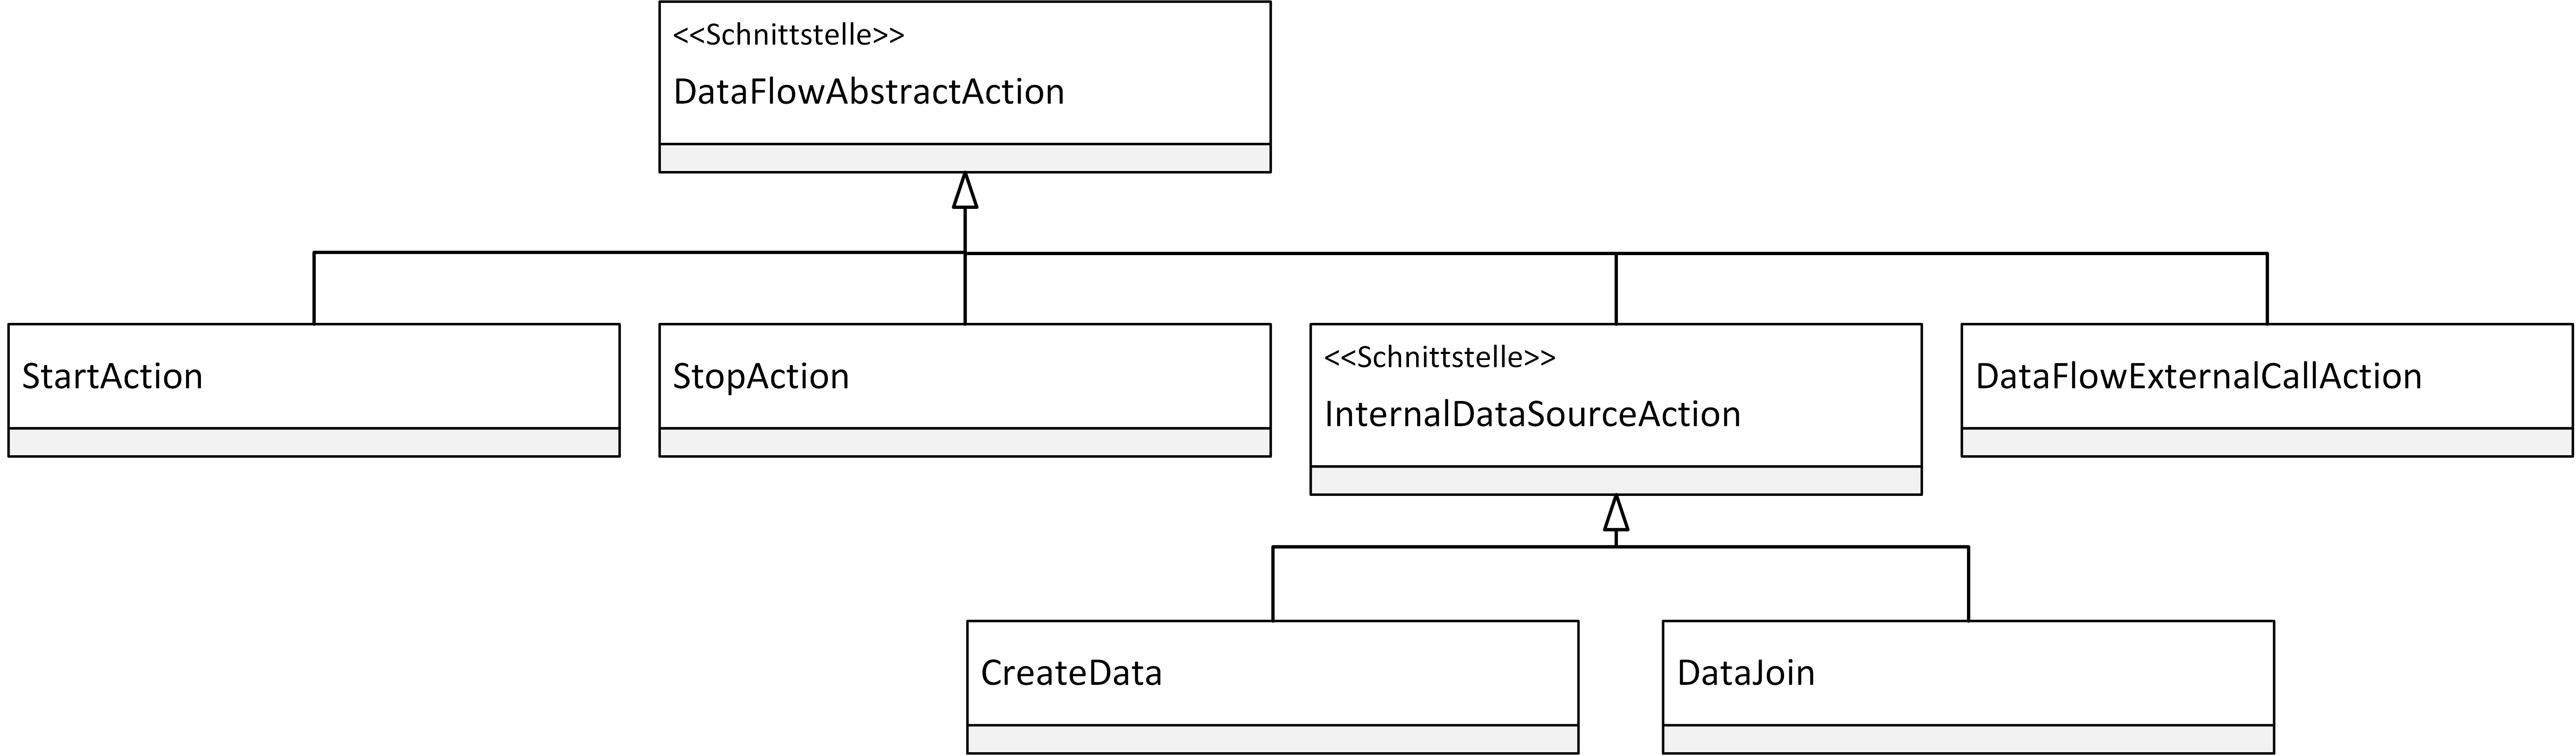
\includegraphics[width=1\textwidth]{images/meta_dfseff_actions.png}
	\caption{Übersicht der Aktionen des DFSEFF}
	\label{img:modell:dfseff:actions}
\end{figure}
Das wohl wichtigste Konzept des \gls{dfseff} ist die Möglichkeit Daten und Parameter zu verknüpfen. Dadurch können Daten durch das System verfolgt werden und schließlich in \texttt{DataSet}s eingeordnet werden. Die Modellierung dazu ist in \autoref{img:modell:dfseff:bindings} abgebildet. Mithilfe des Elements \texttt{VariableBinding} können \texttt{DataFlowExternalAction}s um eine Verknüpfung von Daten und Parameter erweitert werden. Diese Verknüpfung wird als \texttt{Binding} modelliert. Ein \texttt{Binding} besteht aus einem Parameter, der aus einer Signatur stammt, die die \texttt{DataFlowExternalAction} aufruft und einer Datenklasse. \texttt{Binding}s werden in \texttt{BindingContainer} gesammelt und gruppiert. \par
\begin{figure}[h]
	\centering
  	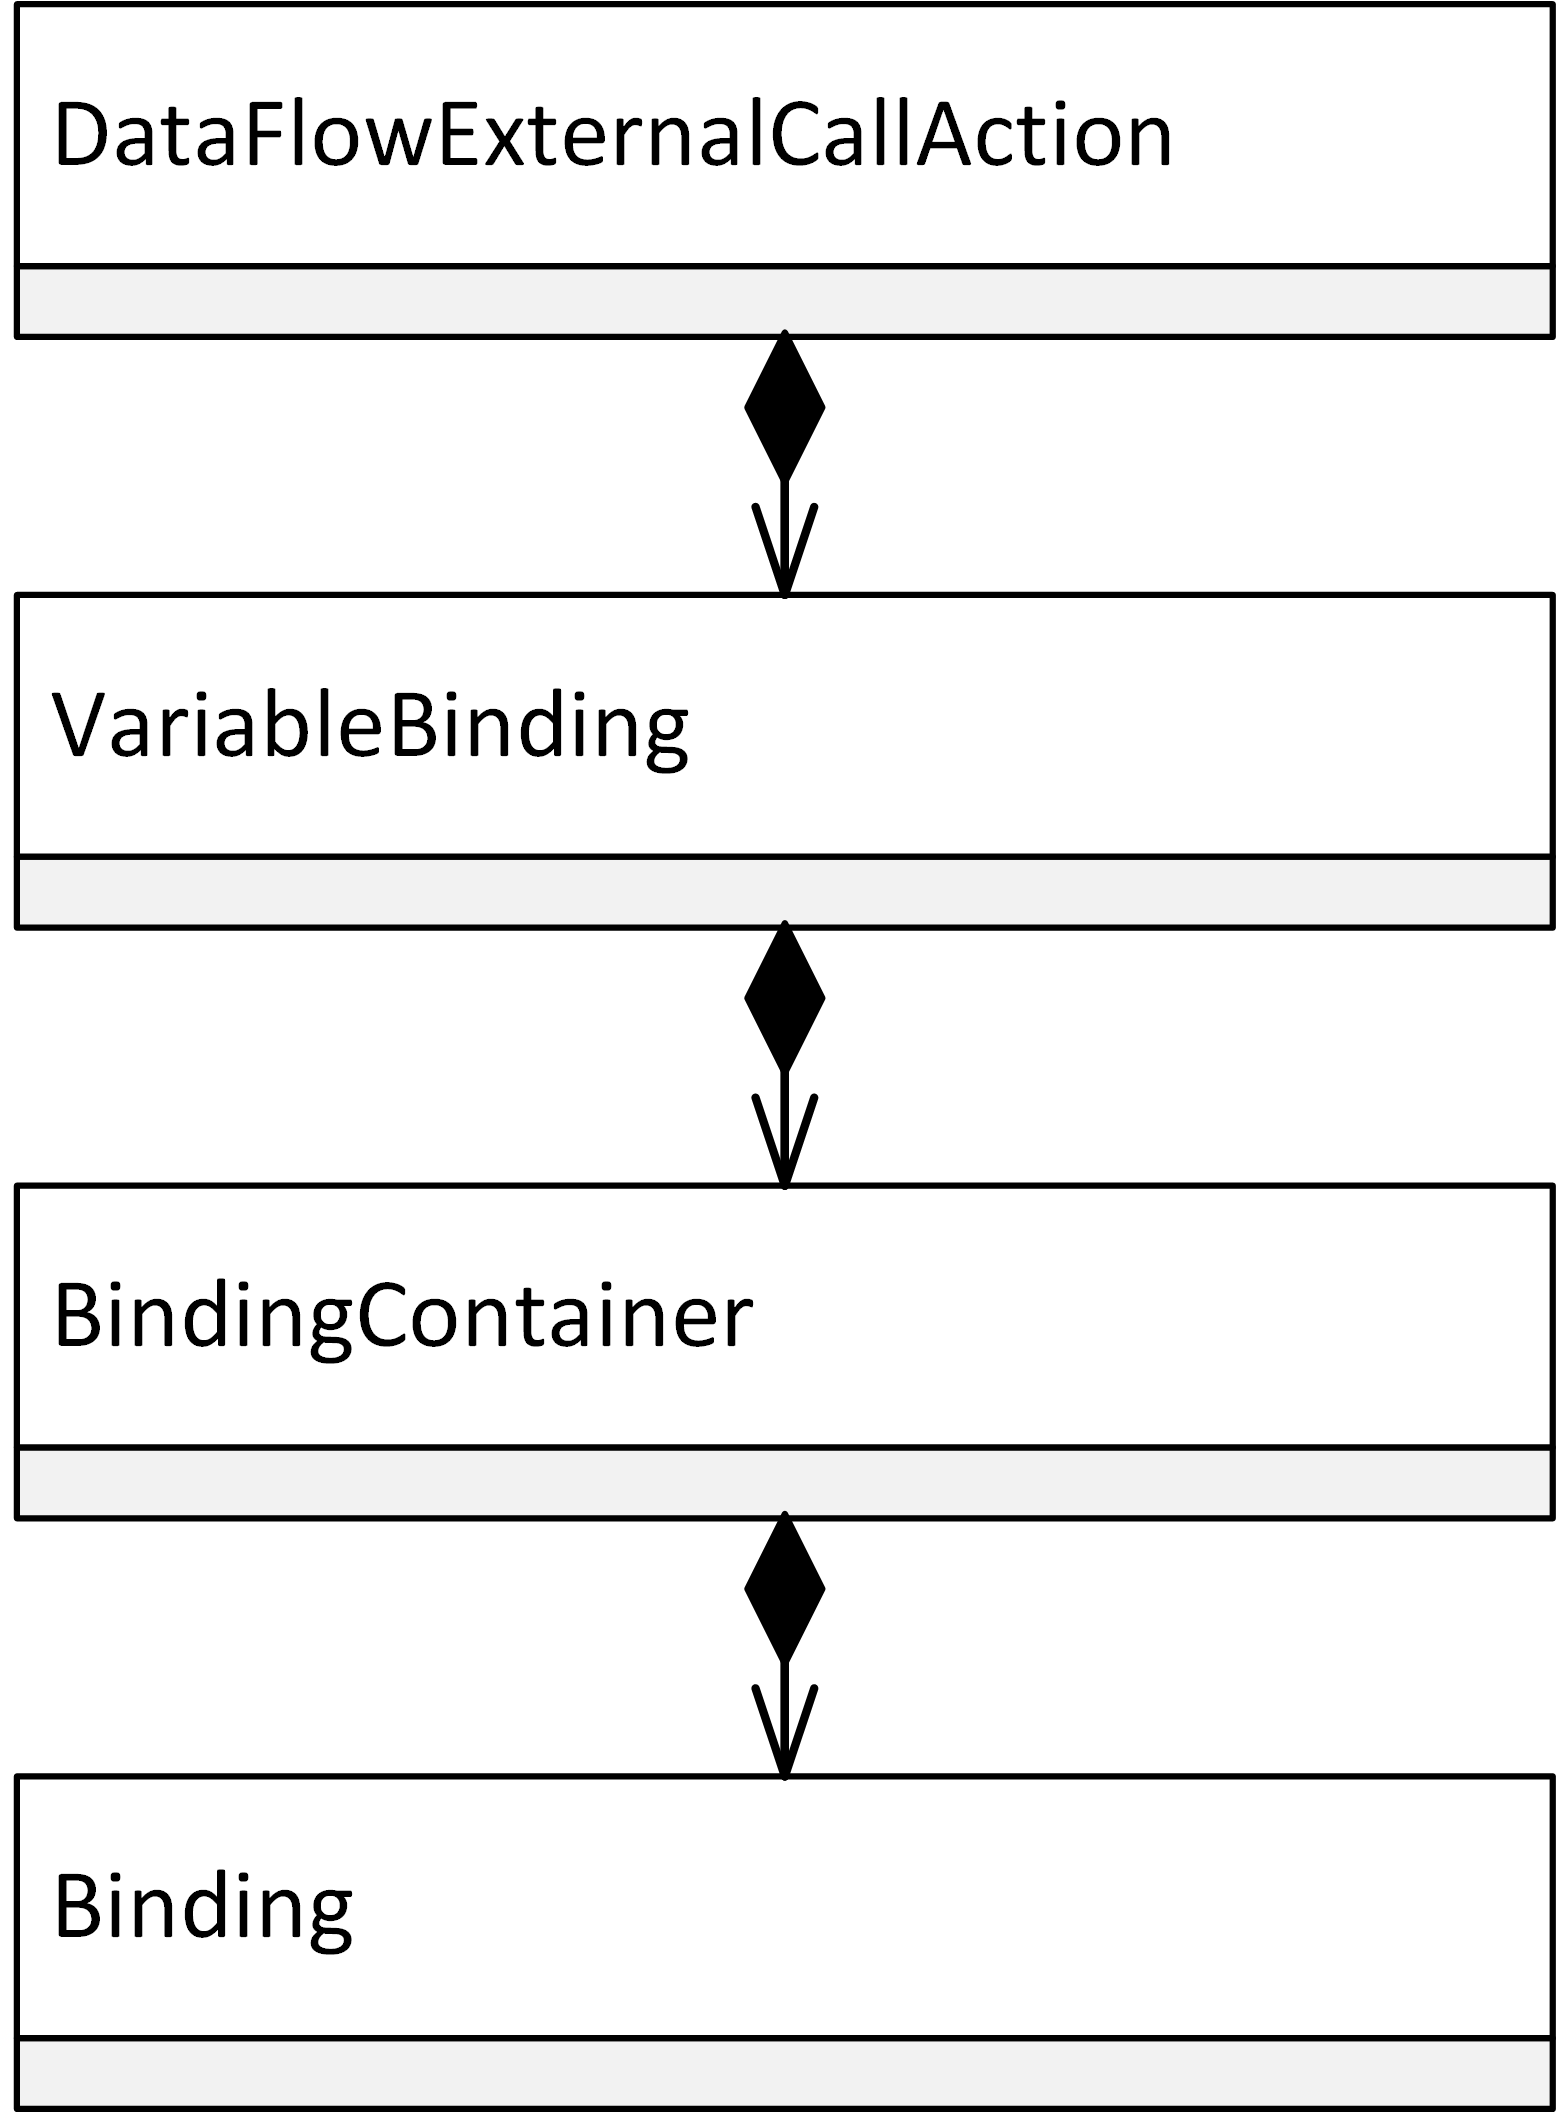
\includegraphics[width=0.35\textwidth]{images/meta_dfseff_bindings.png}
	\caption{Übersicht der Modellierung von \texttt{Binding}s}
	\label{img:modell:dfseff:bindings}
\end{figure}
In \autoref{img:szenario:seff} wurde der Datenfluss des Kaufvorgangs aus \autoref{sec:szenario} als \gls{dfseff} modelliert. In dieser Modellierung gibt es die Datenklasse \textit{ProductData}. Der Datenfluss fängt mit einer \texttt{DataFlowExternalAction} an, die den Dienst \texttt{checkForProduct(Product product)} aufruft. Sie enthält ein \texttt{Binding}, das den Parameter \textit{product} mit der Datenklasse \textit{ProductData} verknüpft. Als nächstes wird eine weitere \texttt{DataFlowExternalAction} ausgeführt. Sie ruft den Dienst \texttt{getProduct(Product product)} auf. Diese Aktion enthält ebenfalls ein \texttt{Binding}. Dieses verknüpft den Parameter \textit{product} mit der Datenklasse \textit{ProductData}. Schließlich wird mit \texttt{CreateData} ein neues Datum erstellt. Das neue Datum heißt \textit{Product}. Mit dieser letzten Aktion endet der Datenfluss.

\begin{figure}[h]
	\centering
  	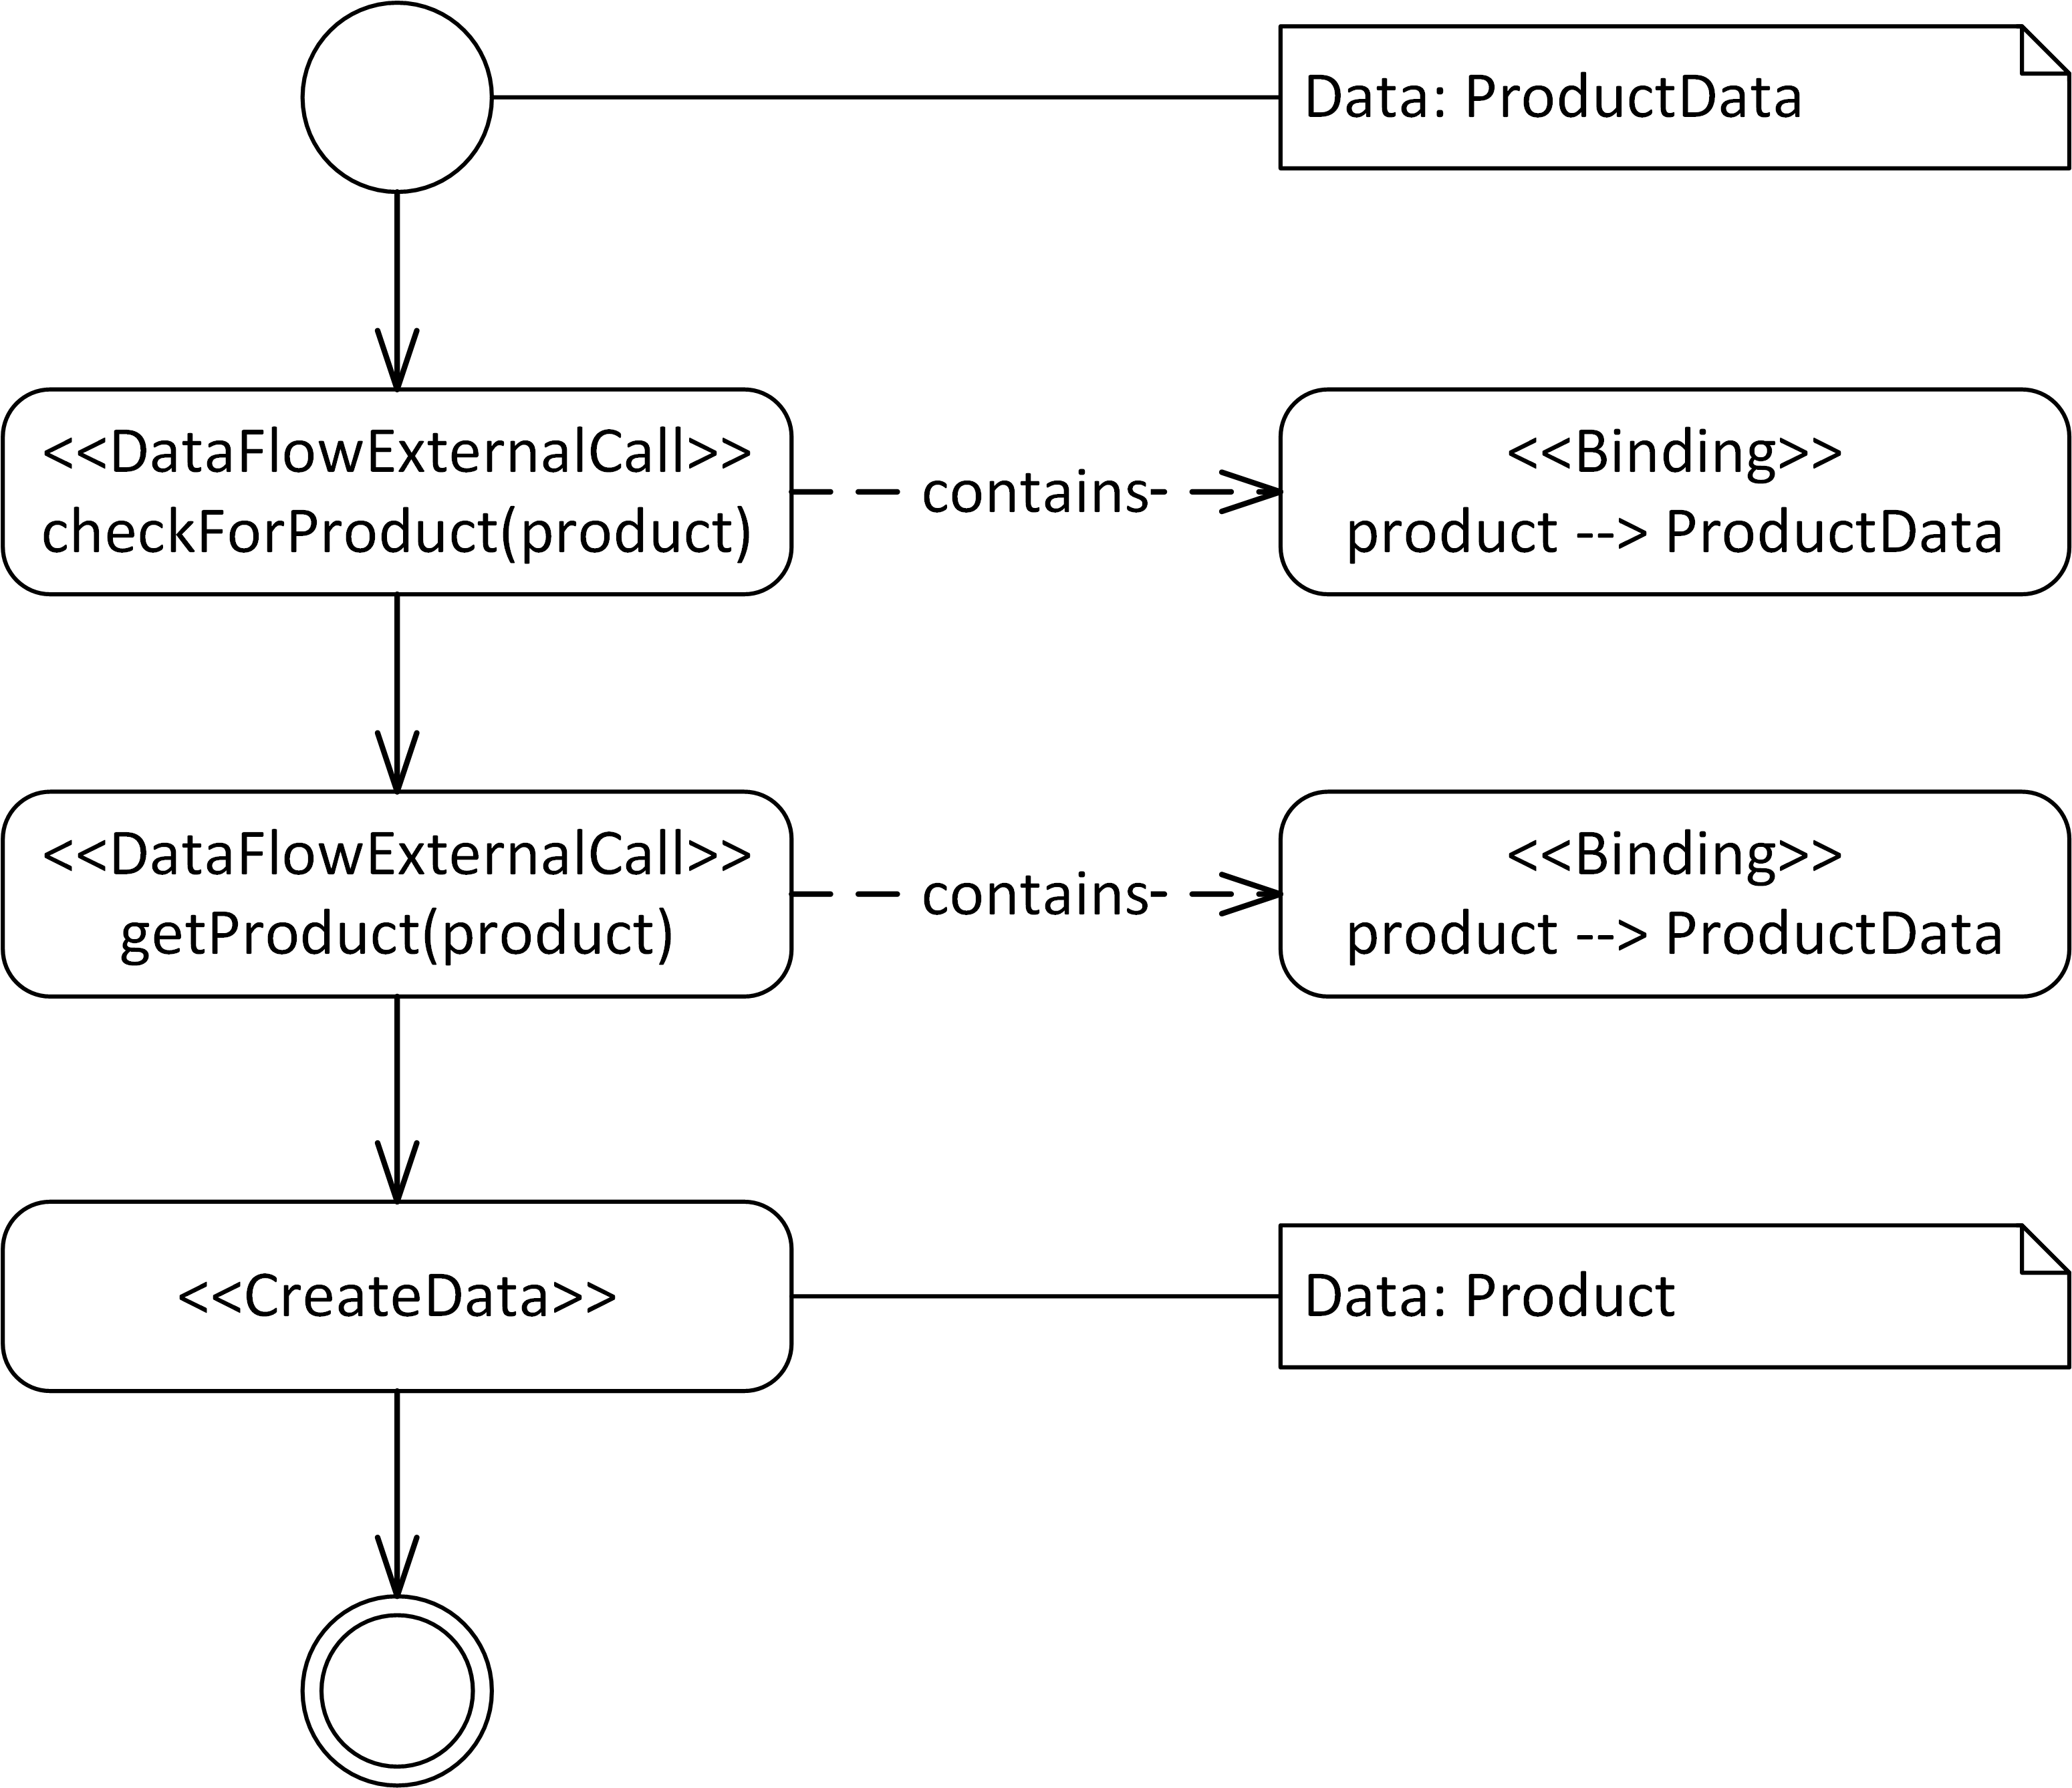
\includegraphics[width=0.7\textwidth]{images/szenario_seff.png}
	\caption{Datenfluss des Dienstes \texttt{buy(Product product)} aus dem Laden-Szenario}
	\label{img:szenario:seff}
\end{figure}

\section{Domänenexperte}
\label{sec:paket:usage}
Diese Erweiterung ermöglicht es, dem Domänenexperten, den Datenfluss im Nutzungsmodell zu modellieren. Die Erweiterung ist ähnlich aufgebaut wie die Erweiterung des Komponentenentwickler aus \autoref{sec:paket:dfseff}. Für die Modellierung wurden hier zwei Ansätze identifiziert. Zunächst wurde festgestellt, dass das Element \texttt{AbstractUserAction}, aus dem \gls{pcm}, nicht \gls{rdseff} spezifisch ist und deshalb wiederverwendet werden kann. \texttt{AbstractUserAction} ist vergleichbar zu der \texttt{AbstractAction} und modelliert einen Aufruf zu einem Dienst, der von einem Benutzer getätigt wird. Der erste Ansatz wäre einen \texttt{DataFlowEntryLevelSystemCall}, ähnlich dem \texttt{EntryLevelSystemCall} aus Palladio, zu definieren. Der \texttt{EntryLevelSystemCall} modelliert einen Aufruf zu einem Dienst, der von einem PCM-System bereitgestellt wird. Dieser \texttt{DataFlowEntryLevelSystemCall} hätte \\ \texttt{AbstractUserAction} als Basisklasse und würde zusätzlich \texttt{Binding}s enthalten. Dieser Ansatz hätte jedoch den Nachteil, dass der Domänenexperte bereits modellierte \texttt{EntryLevel-\\SystemCall}s nochmal modellieren müsste, um den Datenfluss zu berücksichtigen. Der zweite Ansatz, der realisiert wurde, ist in \autoref{img:modell:usage} abgebildet. Dabei wird das Nutzungsmodell um das Elemente \texttt{UsageVariableBinding} erweitert. \texttt{UsageVariableBinding} besitzt als Basisklasse das Element \texttt{VariableBinding} aus \autoref{sec:paket:dfseff}. \texttt{UsageVariable-\\Binding} hat eine Referenz auf einen \texttt{EntryLevelSystemCall} aus dem \gls{pcm}. Diese Referenz ist möglich, da der \texttt{EntryLevelSystemCall} nicht abhängig vom \gls{rdseff} ist. Somit wurden auch in diesem Ansatz  Elemente wiederverwendet. Außerdem hat der Benutzer weniger Modellierungsaufwand, da er bereits modellierte \texttt{EntryLevelSystemCall}s wiederverwenden kann. Signaturen können auch hier wiederverwendet werden, denn die Daten müssen auch vom Benutzer in das System gelangen. Das Root-Element dieser Erweiterung ist das Element \texttt{UsageModelContainer}. Es enthält die \texttt{UsageVariableBinding}s, die für die Modellierung des Datenflusses im Nutzungsmodell verwendet werden. \par
\begin{figure}[h]
	\centering
  	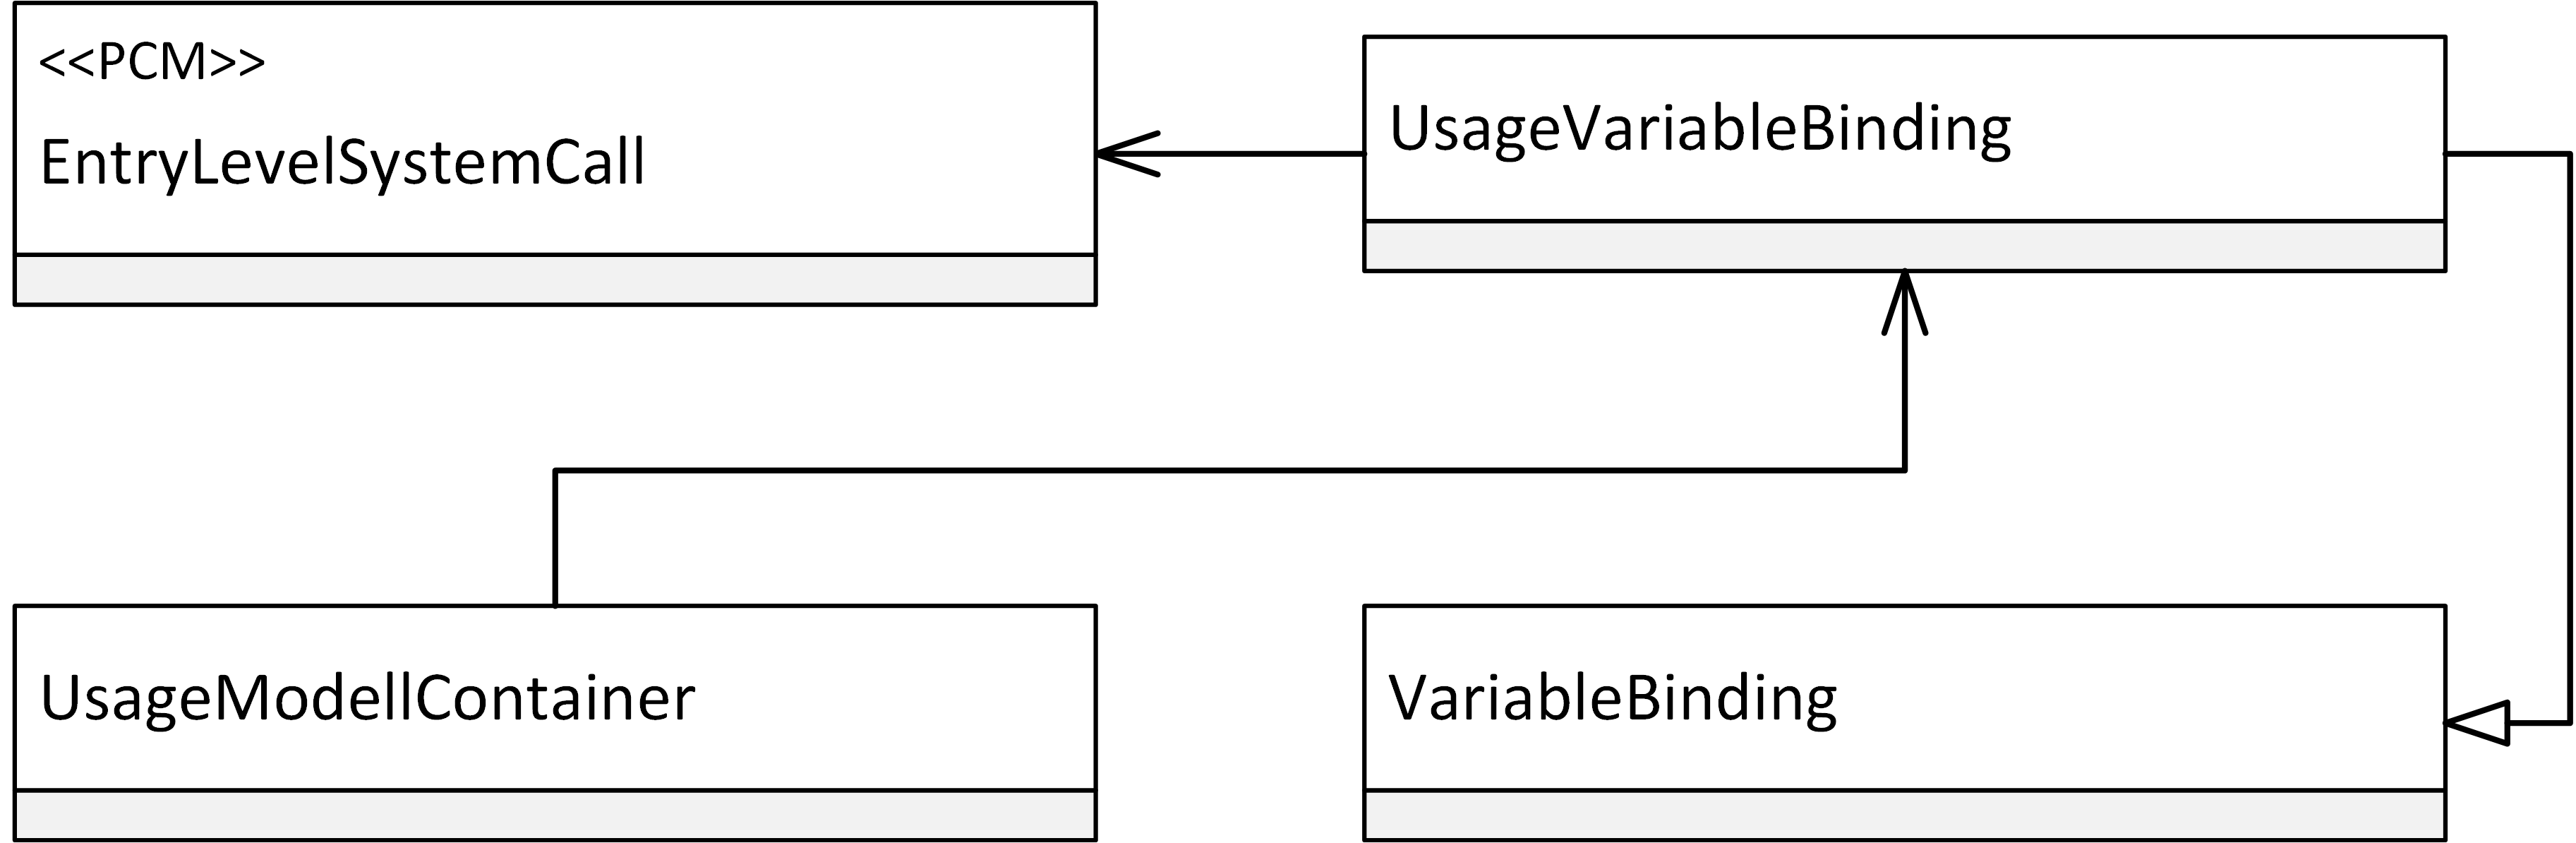
\includegraphics[width=0.85\textwidth]{images/meta_usage.png}
	\caption{Modellierung der Erweiterung für das Nutzungsmodell}
	\label{img:modell:usage}
\end{figure}
In \autoref{img:szenario:usage} ist der Datenfluss im Nutzungsmodell, anhand des Beispiels aus \autoref{sec:szenario}, modelliert. In der Modellierung gibt es die Datenklassen \textit{ProductData} und \textit{CreditCardData}. Der Datenfluss beginnt mit einem \texttt{EntryLevelSystemCall}, der den Dienst \texttt{buy(Product product)} aufruft. Außerdem wird er von einem \texttt{UsageBinding}, dass den Parameter \textit{product} mit der Datenklasse \textit{ProductData} verknüpft, referenziert. Die Daten fließen zum Nächsten \texttt{EntryLevelSystemCall}, welcher wiederum den Dienst \texttt{pay(CreditCard creditCard)} aufruft. Auch dieser \texttt{EntryLevelSystemCall} wird von einem \texttt{UsageBinding}, dass den Paramter \textit{creditCard} mit der Datenklasse \textit{CreditCardData} verknüpft, referenziert. Danach endet der Datenfluss.

\begin{figure}[h]
	\centering
  	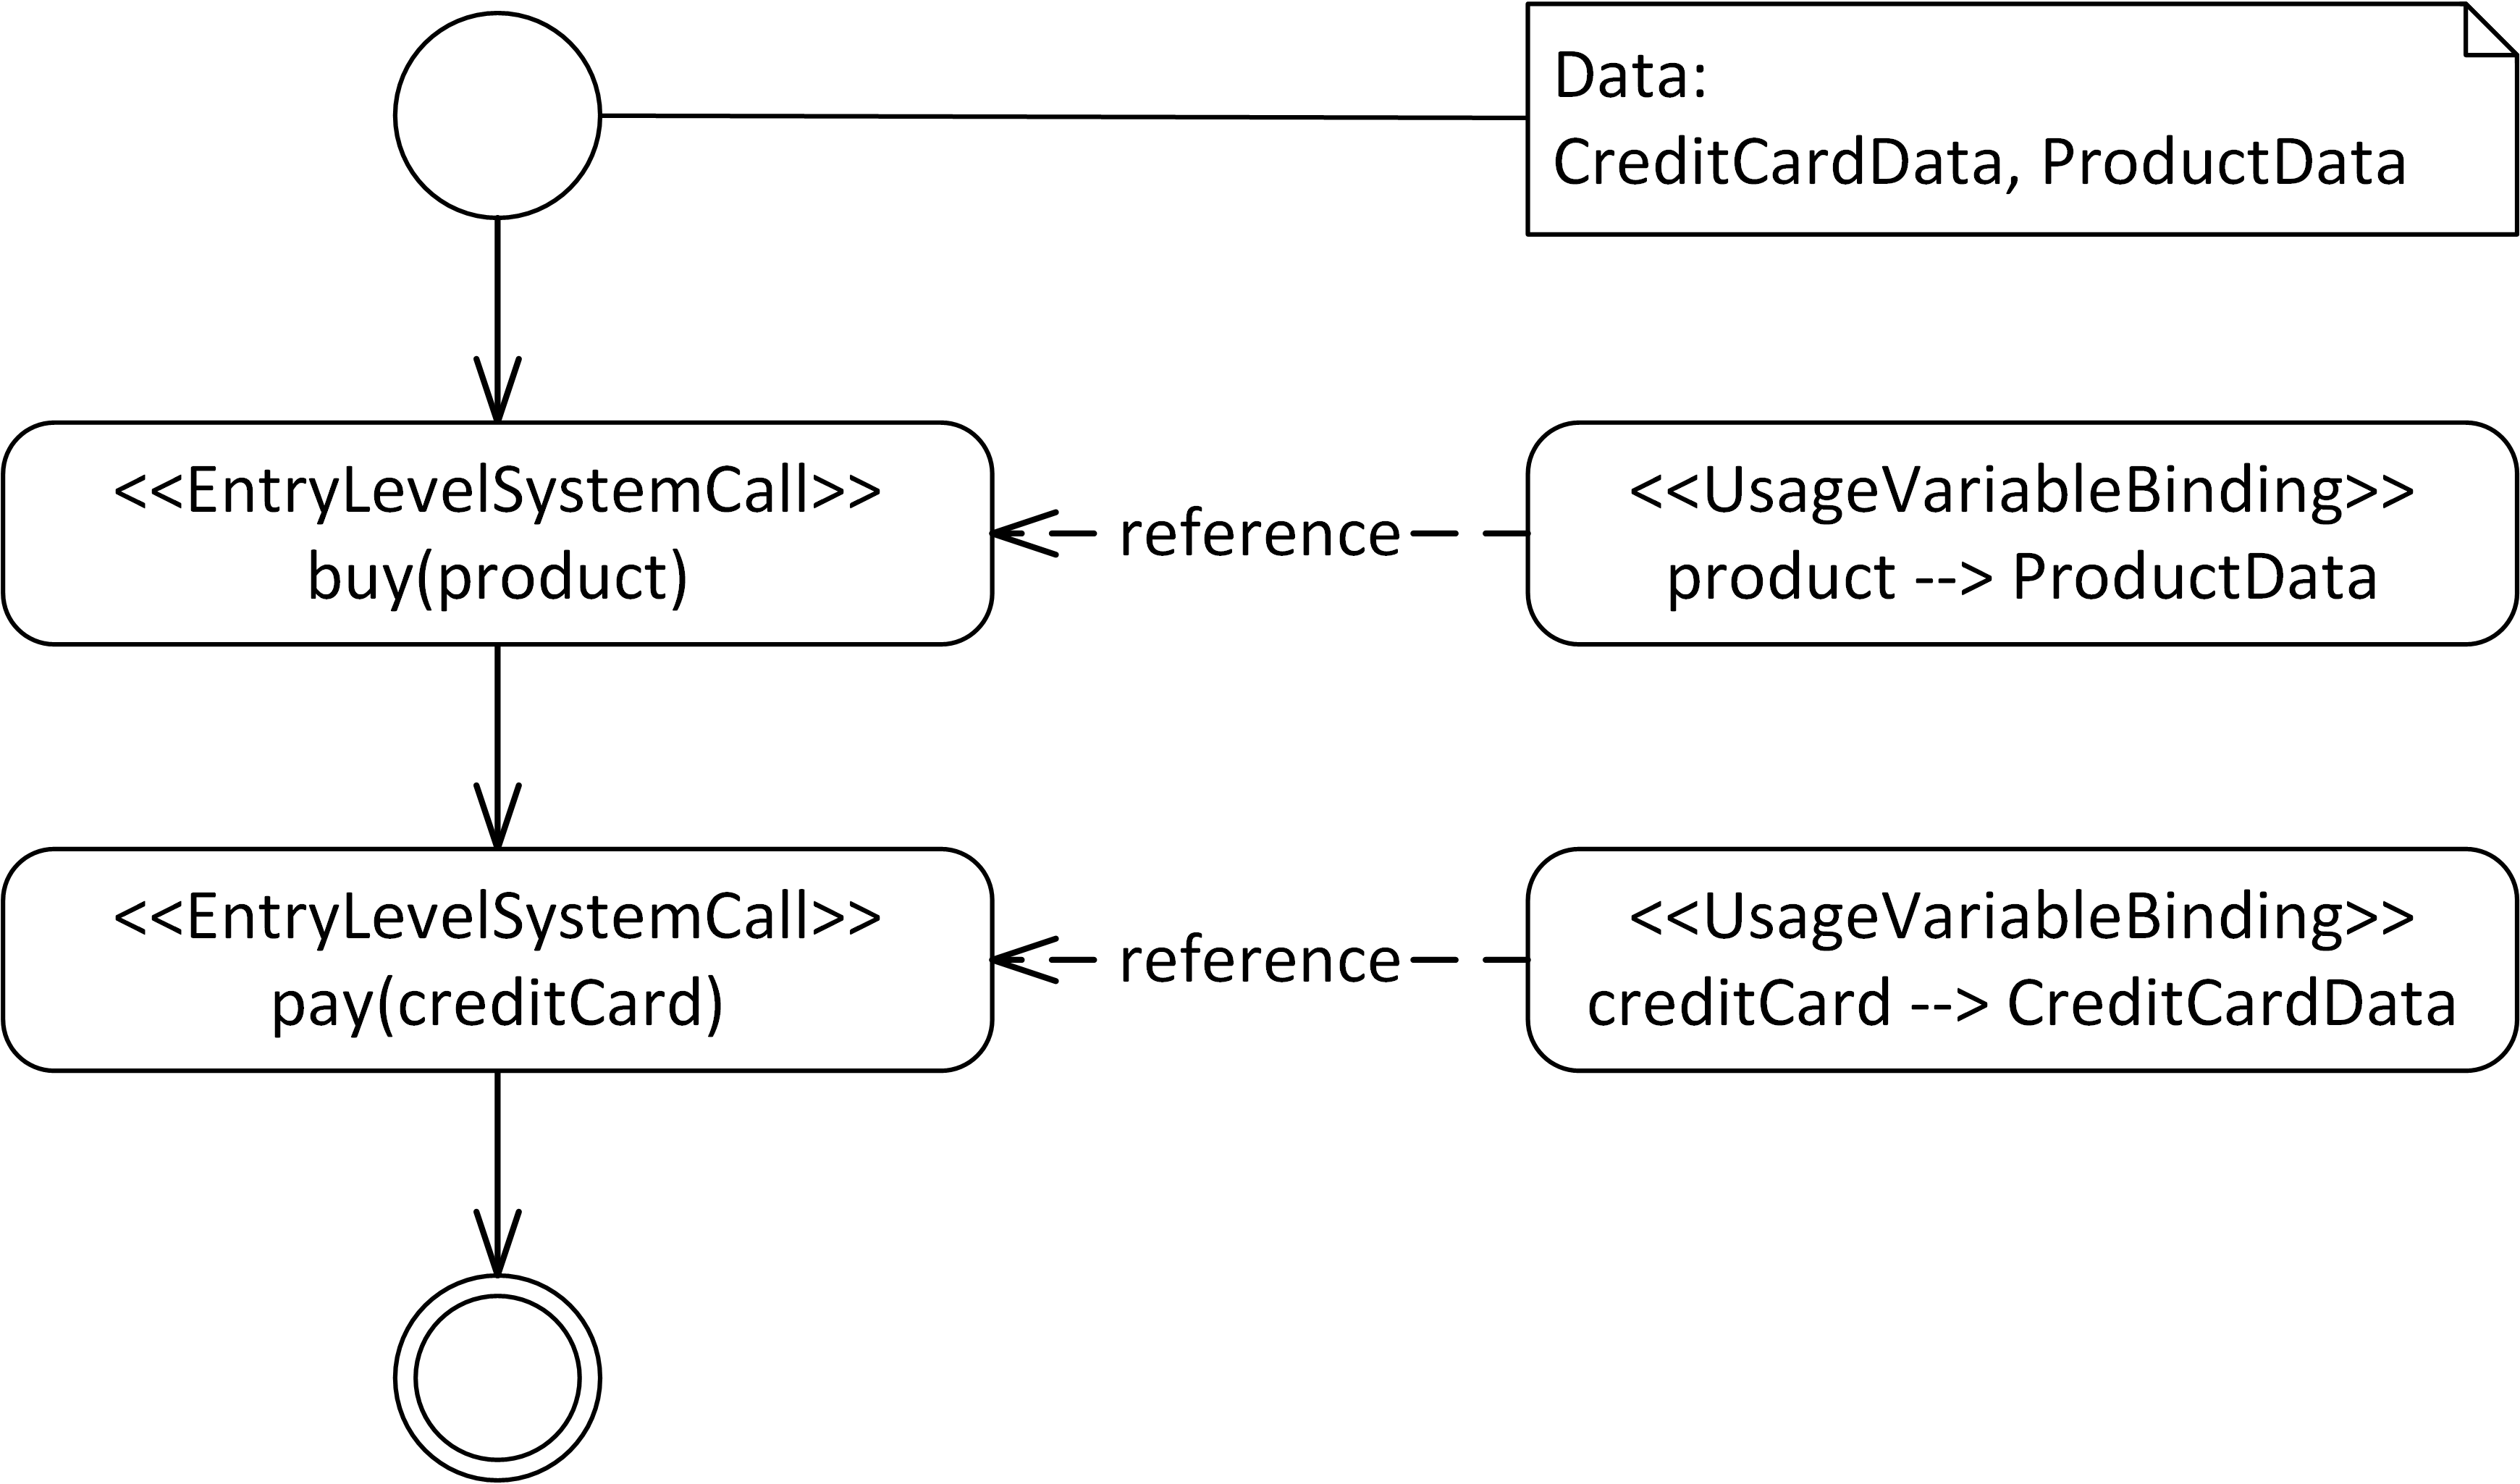
\includegraphics[width=0.85\textwidth]{images/szenario_usage.png}
	\caption{Datenfluss, der vom Benutzer ausgeht}
	\label{img:szenario:usage}
\end{figure}